\documentclass[a4paper]{article}
%===================================================
\pdfoptionpdfminorversion=7
%===================================================
\usepackage{etex}
\usepackage[top=2.5cm,bottom=3cm,left=3cm,right=2.5cm,headsep=24pt,footskip=32pt,a4paper]{geometry}
\usepackage{booktabs,tabularx}
\RequirePackage[T1]{fontenc}
\RequirePackage[utf8]{inputenc}
\RequirePackage[spanish,english,es-nodecimaldot]{babel}
%===================================================
\RequirePackage{fontawesome5}
\RequirePackage[x11names,usenames,dvipsnames,svgnames,table]{xcolor}
\RequirePackage[full]{textcomp}
\RequirePackage{esvect,amsmath,amsthm,amssymb,amsfonts,latexsym,cancel,stmaryrd}
\RequirePackage{setspace}
\parindent= 0mm
\clubpenalty= 10000
\widowpenalty= 10000
\displaywidowpenalty= 10000
\renewcommand{\baselinestretch}{1.3}
\RequirePackage{anyfontsize}
\RequirePackage{etoolbox}
\RequirePackage{titlesec}
\RequirePackage{titletoc}
\RequirePackage[nottoc]{tocbibind}
\RequirePackage{ifthen}
\titlespacing{\section}{0pt}{12pt}{2pt}
\titlespacing{\subsection}{0pt}{12pt}{2pt}
\titlespacing{\subsubsection}{0pt}{12pt}{2pt}
\titlespacing{\paragraph}{0pt}{12pt}{2pt}
\titleformat{\paragraph}[hang]%[block]
	{\setlength{\parskip}{0pt}\bfseries\normalsize\selectfont}%
	%{\makebox[0.8cm][l]{\daxx{m}{n}\fontsize{11pt}{11pt}\selectfont\thesubsection\,.}}
	{}
	{0em}
	{\vphantom{2}}
\setcounter{secnumdepth}{4}
\setcounter{tocdepth}{3}

\dottedcontents{section}[1.6em]{\bfseries}{1.3em}{.6em}

%----------------------------------------------------------------------------------------------------

\RequirePackage{rotating}
\RequirePackage{pdflscape}
\RequirePackage{bookmark}
\RequirePackage{tikz}
\usetikzlibrary{babel}
\RequirePackage[export]{adjustbox}
\usetikzlibrary{shadows}
\RequirePackage{booktabs}
\RequirePackage{longtable}
\RequirePackage{multirow}
\RequirePackage{multicol}
\setlength\columnseprule{0.5pt}
\RequirePackage{array}
\RequirePackage{tabularx}
\RequirePackage[rflt]{floatflt}
\RequirePackage{enumitem}
\setlist[itemize]{itemsep=-1.5mm,topsep=-5pt,partopsep=9pt}
\setlist[description]{itemsep=-1.5mm,topsep=-1pt,parsep=5pt,partopsep=9pt}
\setlist[enumerate]{itemsep=-1.5mm,topsep=-5pt,partopsep=9pt}
%\setlist[itemize,1]{label=\leavevmode\hbox{} to 1.2ex{\hss\vrule height .9ex width .7ex depth -.2ex\hss}}

\RequirePackage{listings}
\RequirePackage{listingsutf8}
\newcommand{\thess}{%
\renewcommand{\contentsname}{Índice general}
\renewcommand{\partname}{Parte}
\renewcommand{\appendixname}{Anexo}
\renewcommand{\figurename}{Figura}
\renewcommand{\tablename}{Tabla}
\renewcommand{\lstlistingname}{Código}
\renewcommand{\chaptername}{Capítulo}
\renewcommand{\bibname}{Referencias bibliográficas}
\renewcommand\indexname{Índice alfabético}
\renewcommand\listfigurename{Índice de figuras}
\renewcommand\listtablename{Índice de tablas}
\renewcommand\lstlistlistingname{Índice de códigos}
\gdef\thelstlisting{\arabic{section}.\arabic{lstlisting}}
}

%----------------------------------------------------------------------------------------------------

\RequirePackage{blkarray}
\RequirePackage{makecell}
\RequirePackage{cellspace}
\RequirePackage{hhline}
\RequirePackage{color}
\RequirePackage{environ}
\RequirePackage{pdfpages}
\RequirePackage{float}
\RequirePackage{subfig}
\RequirePackage{graphicx}
\RequirePackage{wrapfig}
\usepackage{chngcntr}
\counterwithout{table}{section}
\counterwithout{figure}{section}
%\numberwithin{figure}{section}

%----------------------------------------------------------------------------------------------------

\definecolor{lightgray}{cmyk}{0.00,0.00,0.00,0.05}
\definecolor{ocre}{RGB}{243,102,25}
\definecolor{Azul}{cmyk}{1,0.69,0,0.09}
\definecolor{Crema}{cmyk}{0,0.0172,0.25,0.0902}
\definecolor{Sec1}{cmyk}{0.11,0,0.07,0.29}
\definecolor{Sec2}{cmyk}{1,0,0.46,0.15}
\definecolor{Ncap1}{cmyk}{0,1,,0.8,0.02}
\definecolor{Fcap1}{cmyk}{0,0,0,0.14}
\definecolor{Secn1}{cmyk}{1,0,0.55,0.05}
\definecolor{Secn2}{cmyk}{0.90,0.11,0,0}
\definecolor{Secn3}{cmyk}{36,100,0,0}
\definecolor{Celeste}{cmyk}{1,0,0,0.05}
\definecolor{Azul1}{cmyk}{1,0.44,0,0}
\definecolor{Def01}{cmyk}{100,20,0,0}
\definecolor{ContorTeo}{RGB}{74,0,148}
\definecolor{morado01}{RGB}{85,3,250}
\definecolor{morado02}{RGB}{252,3,231}
\definecolor{azul01}{RGB}{0,69,252}
\definecolor{azultwo}{RGB}{18,78,185}
\definecolor{azultre}{RGB}{5,98,200}
\definecolor{azulfor}{RGB}{0,136,206}
\definecolor{rojo01}{RGB}{234,13,44}
\definecolor{resal01}{rgb}{0.77,0.05,0.20}
\definecolor{resal02}{rgb}{0.66,0.04,0.79}
\definecolor{shadecolor}{RGB}{224,238,238}
\definecolor{codmatlab}{rgb}{0.83,0.05,0.25}
\definecolor{chapt}{RGB}{0,143,148}
\definecolor{sayytbcon}{RGB}{204,204,205}
\definecolor{sayytbcell}{RGB}{245,246,246}
\definecolor{minicont}{rgb}{0.99,0.81,0.09}
\definecolor{azzul}{RGB}{6,96,167}
\definecolor{azzul01}{RGB}{252,250,222}
\definecolor{ruddy}{rgb}{1.0, 0.0,0.16}
\definecolor{bubbles}{rgb}{0.91, 1.0,1.0}
\definecolor{mediumpersianblue}{rgb}{0.0, 0.4, 0.65}
\definecolor{gainsboro}{rgb}{0.86,0.86, 0.86}
\definecolor{groupcod}{RGB}{103, 140, 177}
\definecolor{groupllv}{RGB}{0, 43, 54}
\definecolor{coddfond}{rgb}{1.00,1.00,0.91}
\definecolor{coddlin}{rgb}{0.00,0.62,0.62}
\definecolor{blau}{RGB}{17,94,140}
\definecolor{lemonchiffon}{rgb}{1.0,0.98, 0.8}
\definecolor{purpleheart}{rgb}{0.41,0.21, 0.61}
\definecolor{richcarmine}{rgb}{0.84,0.0, 0.25}
\definecolor{raspberry}{rgb}{0.89,0.04, 0.36}
\definecolor{groupcorch}{RGB}{0, 82, 102}
\definecolor{grverd}{rgb}{.133,.545,.133}
\definecolor{itfold}{rgb}{0.81,0.57,0.00}
\definecolor{darkturquoise}{RGB}{0, 206, 209}
\definecolor{turquoiseblue}{RGB}{0, 199, 140}
\definecolor{azzulverde}{RGB}{0,112,131}
\definecolor{miverde}{RGB}{44,162,67}
\definecolor{graylite}{RGB}{206, 206, 206}
\definecolor{azulicg}{RGB}{3, 24, 61}
\definecolor{azzulcont}{RGB}{8,8,123}
\definecolor{trueblue}{rgb}{0.0, 0.45, 0.81}
\definecolor{gold}{RGB}{255,198,0}
\definecolor{azulunsch}{RGB}{2,65,119}
\definecolor{rojomio}{RGB}{220,10,99}
% colores HTML
\definecolor{bblue}{HTML}{4F81BD}
\definecolor{rred}{HTML}{C0504D}
\definecolor{ggreen}{HTML}{9BBB59}
\definecolor{ppurple}{HTML}{9F4C7C}
\RequirePackage{fancyhdr}

%----------------------------------------------------------------------------------------------------

\DeclareCaptionLabelSeparator{syfsepAPAt}{\quad}
\DeclareCaptionFont{cfblack}{\color{black}}
\DeclareCaptionFont{sybf}{\fontsize{10pt}{14pt}\selectfont\bfseries}
\DeclareCaptionFont{synfapat}{\fontsize{10pt}{14pt}\itshape\selectfont}%
\DeclareCaptionFormat{sybformat}%
{#1#2\par\vspace*{-6pt}\parbox[t]{\linewidth}{\itshape#3}}%
\usepackage{caption}
\captionsetup{format=hang,justification=justified}
\captionsetup[lstlisting]{labelfont={cfblack,bf},textfont={cfblack},skip=0pt,aboveskip=5pt,belowskip=0pt}
\captionsetup[listing]{labelfont={cfblack,bf},textfont={cfblack},skip=0pt,aboveskip=0pt,belowskip=0pt}
\captionsetup[figure]{format=sybformat,margin=0mm,skip=6pt,labelsep=syfsepAPAt,labelfont={cfblack,sybf},textfont={cfblack,synfapat},indention=0pt,belowskip=0pt}
\captionsetup[table]{format=sybformat,margin=0mm,skip=6pt,labelsep=syfsepAPAt,labelfont={cfblack,sybf},textfont={cfblack,synfapat},indention=0pt,belowskip=0pt}
%=================================
\DeclareCaptionFormat{syapafformat}{#1#2\,#3}
\DeclareCaptionLabelSeparator{syfsep}{:\space}
\captionsetup[figure]{format=syapafformat,margin=0mm,skip=6pt,labelsep=syfsep,labelfont={cfblack,sybf},textfont={cfblack},indention=0pt,belowskip=0pt,name={Fig.}}
%=================================
%\DeclareCaptionFormat{syapafformatz}{#1#2\,\,#3}
%\DeclareCaptionLabelSeparator{syfsepAPAf}{:}
%\DeclareCaptionFont{synf}{\normalfont\selectfont}
%\captionsetup[figure]{format=syapafformatz,margin=0mm,skip=6pt,labelsep=syfsepAPAf,labelfont={cfblack,sybf},textfont={cfblack,synf},indention=0pt,belowskip=0pt}

%\gdef\thefigure{\arabic{figure}}
%\gdef\thetable{\arabic{table}}
\usepackage{amsmath}

\RequirePackage{hyperref}

\tikzstyle{abstractbox} = [draw=black, fill=white, rectangle,
inner sep=10pt, style=rounded corners=5pt, drop shadow={fill=black,
opacity=0.2}]
\newcommand{\boxabstractd}[3][]{%
\par\medskip
\begin{center}
  \begin{tikzpicture}
    \node [abstractbox, #1,inner sep=10pt] (box)
    {\begin{minipage}{#2}
         #3%\footnotesize
      \end{minipage}};
  \end{tikzpicture}
\end{center}}

%===================================================
\lstset{%
  frame=shadowbox,framexleftmargin=7mm, xleftmargin=7mm, xrightmargin=1mm, framexrightmargin=0mm,framextopmargin=0mm,belowcaptionskip=0.5\baselineskip,
  rulesepcolor=\color{gray!65},
	rulecolor=\color{gray},
	numbersep=3mm,%2
    numbers=left,%
    numberstyle=\color{codmatlab}\fontfamily{phv}\tiny,
	breaklines=true,breakatwhitespace=true}

\lstdefinestyle{sycoddpython}{%
    belowcaptionskip=0.5\baselineskip,
	framexleftmargin=1mm,
	xleftmargin=2mm,
	inputencoding=utf8/latin1,
	inputencoding=utf8,
	numbers=left,%none
	numberstyle=\color{codmatlab}\fontfamily{phv}\tiny,%
	stepnumber=1,%
	numbersep=10pt,%
	tabsize=2,%
%	escapeinside={(*@}{@*)},
%	breakatwhitespace=true,
%	backgroundcolor=\color{green!1},
	showstringspaces=false,
	showspaces=false,
	showtabs=false,
	language=Python,
%	basicstyle=\ttfamily\footnotesize,
%	basicstyle={\lstbasicfont},
	basicstyle=\fontencoding{T1}\fontfamily{fvm}\footnotesize\selectfont,%\ttfamily
%	basicstyle={\fontsize{9pt}{11pt}\usefont{T1}{fvm}{m}{n}\selectfont},
%	otherkeywords={self},
	keywordstyle=\color{azultwo}\bfseries,
	keywordstyle= [2]\color{ContorTeo}, % just to check that it works
	emph={MyClass,__init__,AbrirArchivo,VerArchivo},
	emphstyle=\color{morado02},
	emph={[2]from,import,pass,return},
	emphstyle={[2]\color[HTML]{DD52F0}},
	emph={[3]range},
	emphstyle={[3]\color[HTML]{D17032}},
	emph={[4]for,in,def},
	emphstyle={[4]\color{blue}},
	columns=fullflexible,
	prebreak = \mbox{{\color{gray}\tiny$\searrow$}},%
	breaklines=true,
	%inputencoding=utf8,
	extendedchars=true,
	literate=%
      {á}{{\'a}}1  {é}{{\'e}}1  {í}{{\ \@'i}}1 {ó}{{\'o}}1  {ú}{{\'u}}1
      {Á}{{\'A}}1  {É}{{\'E}}1  {Í}{{\'I}}1 {Ó}{{\'O}}1  {Ú}{{\'U}}1
      {à}{{\`a}}1  {è}{{\`e}}1  {ì}{{\ \@`i}}1 {ò}{{\`o}}1  {ù}{{\`u}}1
      {À}{{\`A}}1  {È}{{\'E}}1  {Ì}{{\`I}}1 {Ò}{{\`O}}1  {Ù}{{\`U}}1
      {ä}{{\"a}}1  {ë}{{\"e}}1  {ï}{{\"\@i}}1 {ö}{{\"o}}1  {ü}{{\"u}}1
      {Ä}{{\"A}}1  {Ë}{{\"E}}1  {Ï}{{\"I}}1 {Ö}{{\"O}}1  {Ü}{{\"U}}1
      {â}{{\^a}}1  {ê}{{\^e}}1  {î}{{\ \@^i}}1 {ô}{{\^o}}1  {û}{{\^u}}1
      {Â}{{\^A}}1  {Ê}{{\^E}}1  {Î}{{\^I}}1 {Ô}{{\^O}}1  {Û}{{\^U}}1
      {œ}{{\oe}}1  {Œ}{{\OE}}1  {æ}{{\ae}}1 {Æ}{{\AE}}1  {ß}{{\ss}}1
      {ç}{{\c c}}1 {Ç}{{\c C}}1 {ø}{{\o}}1  {Ø}{{\O}}1   {å}{{\r a}}1
      {Å}{{\r A}}1 {ã}{{\~a}}1  {õ}{{\~o}}1 {Ã}{{\~A}}1  {Õ}{{\~O}}1
      {ñ}{{\~n}}1  {Ñ}{{\~N}}1  {¿}{{?`}}1  {¡}{{!`}}1
      {°}{{\textdegree}}1 {º}{{\textordmasculine}}1 {ª}{{\textordfeminine}}1,
	commentstyle=\color{grverd},
	stringstyle=\color{Sec1},
}

\makeatletter
\def\@copyrightyear{\number\the\year}
\def\@university{UNIVERSIDAD NACIONAL DE SAN CRISTÓBAL DE HUAMANGA}
\def\@faculty{Facultad de Ingeniería de Minas, Geología y Civil}
\def\@dept{Ingeniería Civil}
\def\@teacher{Ing. Edmundo Canchari Gutiérrez}
\def\@course{Métodos Numéricos IC\,-\,343}
\def\@tema{}
\newcommand{\tema}[1]{\renewcommand{\@tema}{#1}}
\newcommand{\dytema}{\@tema}
\def\@email{}
\newcommand{\email}[1]{\renewcommand{\@email}{#1}}
\newcommand{\dyemail}{\@email}
\newcommand{\copyrightyear}[1]{\renewcommand{\@copyrightyear}{#1}}
\newcommand{\university}[1]{\renewcommand{\@university}{#1}}
\newcommand{\faculty}[1]{\renewcommand{\@faculty}{#1}}
\newcommand{\dept}[1]{\renewcommand{\@dept}{#1}}
\newcommand{\course}[1]{\renewcommand{\@course}{#1}}
\newcommand{\teacher}[1]{\renewcommand{\@teacher}{#1}}

\def\@author{David Ramos López}
\def\@title{\empty}
\newcommand{\dycopyrightyear}{\@copyrightyear}
\newcommand{\dyuniversity}{\@university}
\newcommand{\dyfaculty}{\@faculty}
\newcommand{\dydept}{\@dept}
\newcommand{\dycourse}{\@course}
\newcommand{\dyauthor}{\@author}
\newcommand{\dytitle}{\@title}
\newcommand{\dyteacher}{\@teacher}
\newcommand{\@academicyear}{2015- 2016}
\newcommand{\academicyear}[1]{\renewcommand{\@academicyear}{#1}}
\newcommand{\dyacademicyear}{\@academicyear}
\newcommand{\dyyear}{\number\year}
\makeatother
%===================================================
\usepackage[newfloat,section]{minted}
\usemintedstyle{monokai} %perldoc,monokai
\definecolor{bg}{HTML}{282828}
\definecolor{fondoCode}{RGB}{249,249,249}
\definecolor{contorCode}{RGB}{136,0,21}
\definecolor{margenCode}{RGB}{232,202,181}
%*************
\definecolor{fondoCodeE}{RGB}{248,254,254}
\definecolor{contorCodeE}{RGB}{0,162,232}
%*************
\definecolor{fondoCodeNote}{RGB}{248,254,254}
\definecolor{contorCodeNote}{RGB}{0,162,232}

\newcommand{\fondoCodeExerc}{fondoCodeE}
\newcommand{\contorCodeExerc}{contorCodeE}
\newcommand{\ccfondoCodeExerc}[1]{\renewcommand{\fondoCodeExerc}{#1}}
\newcommand{\cccontorCodeExerc}[1]{\renewcommand{\contorCodeExerc}{#1}}

\newcommand{\fondoCodeNote}{fondoCodeE}
\newcommand{\contorCodeNote}{contorCodeE}
\newcommand{\ccfondoCodeNote}[1]{\renewcommand{\fondoCodeNote}{#1}}
\newcommand{\cccontorCodeNote}[1]{\renewcommand{\contorCodeNote}{#1}}


\newcommand{\sen}{\mathop{\rm sen}\nolimits}
\newcommand{\syFv}{\vphantom{\textrm{Í}}}


\makeatletter
\AtBeginDocument{\let\c@listing\c@lstlisting}
\makeatother
\renewcommand{\listingname}{Código}
\newenvironment{longlisting}{\captionsetup{type=listing}}{}

%*********************************************
\usepackage{tcolorbox}
\tcbuselibrary{skins,breakable,listings,minted}
\usetikzlibrary{shapes}
\usetikzlibrary{shapes.misc,calc,positioning}
%-------------------------------------
\tcbuselibrary{theorems}%skins
\usepackage[customcolors,shade]{hf-tikz}

%*********************************************
\newtcblisting{pycode}[6][perldoc]{%
listing engine=minted, minted style=#1, minted language=#2,minted options={framesep=0pt,fontsize=\small,breaklines,numbersep=2mm,#3},listing only, left=5mm,freelance,sharpish corners,enhanced,breakable,boxsep=1mm,right=0mm,top=0mm,bottom=0mm, boxrule=0.7pt,colback=#6,colframe=#4,%
overlay={\begin{tcbclipinterior}\fill[#5] (interior.south west) rectangle ([xshift=5mm]interior.north west);\end{tcbclipinterior}},
% Código para las cajas intactas:
    frame code={%
    \path[draw=#4, line width=0.6pt,fill=#6] (frame.south west)-- (frame.north west)-- (frame.north east)-- (frame.south east)--cycle;
    },
% código para la primera parte de una secuencia de ruptura:
    skin first is subskin of={emptyfirst}{%
    frame code={%
    \path[draw=#4, line width=0.6pt,fill=#6] (frame.south west)-- (frame.north west)-- (frame.north east)-- (frame.south east)--cycle;
    \path[fill=#4] ([xshift=-2.5mm,yshift=1mm]frame.south east)-- + (120:2mm)-- + (60:2mm)-- cycle;
    },
},
% código para la parte media de una secuencia de ruptura:
    skin middle is subskin of={emptymiddle}{%
    frame code={%
    \path[draw=#4, line width=0.6pt,fill=#6] (frame.south west)-- (frame.north west)-- (frame.north east)-- (frame.south east)--cycle;
    \path[fill=#4] ([xshift=-2.5mm,yshift=-1mm]frame.north east)-- + (240:2mm)-- + (300:2mm)-- cycle;
    \path[fill=#4] ([xshift=-2.5mm,yshift=1mm]frame.south east)-- + (120:2mm)-- + (60:2mm)-- cycle;
    },
},
% código de la última parte de una secuencia de ruptura:
    skin last is subskin of={emptylast}{%
    frame code={%
    \path[draw=#4, line width=0.6pt,fill=#6] (frame.south west)-- (frame.north west)-- (frame.north east)-- (frame.south east)--cycle;
    \path[fill=#4] ([xshift=-2.5mm,yshift=-1mm]frame.north east)-- + (240:2mm)-- + (300:2mm)-- cycle;
      },
    },
}
%===================================================

\newtcbinputlisting{\sypycode}[7][perldoc]{%
listing engine=minted, minted style=#1, minted language=#2,minted options={framesep=0pt,fontsize=\small,breaklines,numbersep=2mm,#3},listing only, left=5mm,freelance,sharpish corners,enhanced,breakable,boxsep=1mm,right=0mm,top=0mm,bottom=0mm, boxrule=0.7pt,colback=#6,colframe=#4,%
listing file = {#7},%
overlay={\begin{tcbclipinterior}\fill[#5] (interior.south west) rectangle ([xshift=5mm]interior.north west);\end{tcbclipinterior}},
% Código para las cajas intactas:
    frame code={%
    \path[draw=#4, line width=0.6pt,fill=#6] (frame.south west)-- (frame.north west)-- (frame.north east)-- (frame.south east)--cycle;
    },
% código para la primera parte de una secuencia de ruptura:
    skin first is subskin of={emptyfirst}{%
    frame code={%
    \path[draw=#4, line width=0.6pt,fill=#6] (frame.south west)-- (frame.north west)-- (frame.north east)-- (frame.south east)--cycle;
    \path[fill=#4] ([xshift=-2.5mm,yshift=1mm]frame.south east)-- + (120:2mm)-- + (60:2mm)-- cycle;
    },
},
% código para la parte media de una secuencia de ruptura:
    skin middle is subskin of={emptymiddle}{%
    frame code={%
    \path[draw=#4, line width=0.6pt,fill=#6] (frame.south west)-- (frame.north west)-- (frame.north east)-- (frame.south east)--cycle;
    \path[fill=#4] ([xshift=-2.5mm,yshift=-1mm]frame.north east)-- + (240:2mm)-- + (300:2mm)-- cycle;
    \path[fill=#4] ([xshift=-2.5mm,yshift=1mm]frame.south east)-- + (120:2mm)-- + (60:2mm)-- cycle;
    },
},
% código de la última parte de una secuencia de ruptura:
    skin last is subskin of={emptylast}{%
    frame code={%
    \path[draw=#4, line width=0.6pt,fill=#6] (frame.south west)-- (frame.north west)-- (frame.north east)-- (frame.south east)--cycle;
    \path[fill=#4] ([xshift=-2.5mm,yshift=-1mm]frame.north east)-- + (240:2mm)-- + (300:2mm)-- cycle;
      },
    },
}

%-------------------------------------
\newcommand{\probbkn}[6][0cm]{%
\par\medskip\hspace{#1}
\begin{tikzpicture}[font=\bfseries, every node/.style={signal,%auto,
 signal to=nowhere},remember picture,overlay]%
 \fill[color=#2!10](0cm,0.3cm) rectangle (15.5cm,-0.26cm);
 \fill[color=#2](0cm,0.3cm) rectangle (15.5cm,0.28cm);
 \node[anchor=north west,fill=#2, signal to=east, inner sep=3pt, text=white, drop shadow,line width=1.2pt, draw = #2] at (-0.1,0.3) {\makebox[#3][l]%[l]
 {\hspace{#4}\,#5}};
  \node[text=azzul,line width=0pt] at (10cm,0cm) {\makebox[10.5cm][r]%[l]
 {\normalfont#6}};
\end{tikzpicture}
\par\medskip}
%\probbkn[espacio]{color}{ancho}{espacio}{numero}{libro}\vspace{-5pt}


\newcommand{\nwpar}{\par\vspace{0.3\baselineskip}}

\newcommand\linsecsol[2][-4pt]{\par\vspace{#1}
{\setlength{\parskip}{0pt}\color{#2}\rule[0.5cm]{\textwidth}{1.1pt}}\par\vspace{-0.7cm}}

\newcommand\linseccmdf[3][-4pt]{\par\vspace{#1}
{\color{#3}\rule[0.5cm]{\textwidth}{1.1pt}}\par\vspace{#2}}

\newcommand\sysolution[2][azultwo]{\nwpar%
{\setlength{\parskip}{0pt}\bfseries\color{#1}Solución}\hfill\setlength{\parskip}{0pt}\linseccmdf[0pt]{-0.5cm}{cyan (process)}}

\newcommand\sysolutiont[2][azultwo]{\nwpar%
{\setlength{\parskip}{0pt}\bfseries\color{#1}Solución}\hfill\linsecsol[0pt]{azzul}}

%------------------------------- Cuadro de notas ------------------------------
\tcbset{%
rghstyle/.style={boxsep=1mm,left=1mm,right=1mm,top=1mm,center,before=\par\bigskip,%\centering
    after=\par\medskip,
    breakable,fontupper=\setlength{\parskip}{8pt plus 1pt minus 1pt},
    freelance,
    boxrule=1pt,
% Código para las cajas intactas:
    frame code={%
    \path[draw=\contorCodeNote, line width=0.6pt,fill=\contorCodeNote]
        %([yshift=-7.5pt]frame.north west) -- ([xshift=7.5pt]frame.north west) --
        (frame.north west)-- (frame.north west)--
        (frame.north east)-- (frame.north east|-interior.north east)--
        (frame.north west|-interior.north west)-- cycle;
	%\path[draw=\contorCodeNote!30, line width=20pt] ([xshift=2.25cm,yshift=-10.3pt]frame.north west) --%
	%([xshift=-0.3pt,yshift=-10.3pt]frame.north east);
    },
    interior titled code={
    \path[draw=\contorCodeNote, line width=0.6pt,fill=\fondoCodeNote]
        (frame.west|-interior.north west)-- (frame.east|-interior.north east)--
        (frame.east|-interior.south east)-- (frame.west|-interior.south west)-- cycle;
    \path[anchor=north west,draw=white, line width=1.5pt] ([xshift=-1pt]frame.west|-interior.north west) --%
	([xshift=1pt]frame.east|-interior.north east);
    },
% código para la primera parte de una secuencia de ruptura:
    skin first is subskin of={emptyfirst}{%emptyfirst
    frame code={%
    \path[draw=\contorCodeNote, line width=0.6pt,fill=\contorCodeNote]
        (frame.north west)-- (frame.north west)--
        (frame.north east)-- (frame.north east|-interior.north east)--
        (frame.north west|-interior.north west)-- cycle;
    %\path[draw=\fondoCodeNote,line width=20pt] ([xshift=2.2cm,yshift=-10.3pt]frame.north west) --%
	%([xshift=-0.3pt,yshift=-10.3pt]frame.north east);
	%\path[draw=\contorCodeNote!30, line width=20pt] ([xshift=2.25cm,yshift=-10.3pt]frame.north west) --%
	%([xshift=-0.3pt,yshift=-10.3pt]frame.north east);
    },
    interior titled code={
    \path[draw=\contorCodeNote, line width=0.6pt,fill=\fondoCodeNote]
        (frame.west|-interior.north west)-- (frame.east|-interior.north east)--
        (frame.east|-interior.south east)-- (frame.west|-interior.south west)-- cycle;
    \path[anchor=north west,draw=white, line width=1.5pt] ([xshift=-1pt]frame.west|-interior.north west) --%
	([xshift=1pt]frame.east|-interior.north east);
    },},
% código para la parte media de una secuencia de ruptura:
    skin middle is subskin of={emptymiddle}{%
    frame code={\path[draw=\contorCodeNote, line width=0.6pt, fill=\fondoCodeNote] (frame.south west)--
      (frame.north west)-- (frame.north east)--
      (frame.south east)-- (frame.south east)--cycle;
      },
      },
% código de la última parte de una secuencia de ruptura:
    skin last is subskin of={emptylast}{%
    frame code={\path[draw=\contorCodeNote, line width=0.6pt, fill=\fondoCodeNote] (frame.south west)--
      (frame.north west)-- (frame.north east)--
      (frame.south east)-- (frame.south east)--cycle;
      },
    },
%------------
    fonttitle=\bfseries\vphantom{dy},%
    %fontupper=\sffamily,
},
notehibbstyle/.style={boxsep=1mm,left=1mm,right=1mm,top=1mm,center,before=\par\bigskip,%\centering
    breakable,fontupper=\setlength{\parskip}{8pt plus 1pt minus 1pt},
    freelance,
    boxrule=1pt,
    width=0.98\linewidth,
% Código para las cajas intactas:
    frame code={%
    \path[draw=\contorCodeNote, line width=0.6pt,fill=\contorCodeNote]%\contorCodeNote
        %([yshift=-7.5pt]frame.north west) -- ([xshift=7.5pt]frame.north west) --
        (frame.north west)-- (frame.north west)--
        (frame.north east)-- (frame.north east|-interior.north east)--
        (frame.north west|-interior.north west)-- cycle;
	\path[draw=\fondoCodeNote,line width=20pt] ([xshift=0.65cm,yshift=-10.3pt]frame.north west) --%
	([xshift=-0.3pt,yshift=-10.3pt]frame.north east);
	\path[draw=\contorCodeNote!60, line width=20pt] ([xshift=0.7cm,yshift=-10.3pt]frame.north west) --%
	([xshift=-0.3pt,yshift=-10.3pt]frame.north east);
    },
    interior titled code={
    \path[draw=\contorCodeNote, line width=0.6pt,fill=\fondoCodeNote]
        (frame.west|-interior.north west)-- (frame.east|-interior.north east)--
        (frame.east|-interior.south east)-- (frame.west|-interior.south west)-- cycle;
    \path[draw=white, line width=1.5pt] ([xshift=-1pt]frame.west|-interior.north west) --%
	([xshift=1pt]frame.east|-interior.north east);
    },
% código para la primera parte de una secuencia de ruptura:
    skin first is subskin of={emptyfirst}{%
    frame code={%
    \path[draw=\contorCodeNote, line width=0.6pt,fill=\contorCodeNote]
        (frame.north west)-- (frame.north west)--
        (frame.north east)-- (frame.north east|-interior.north east)--
        (frame.north west|-interior.north west)-- cycle;
	\path[draw=\fondoCodeNote,line width=20pt] ([xshift=0.65cm,yshift=-10.3pt]frame.north west) --%
	([xshift=-0.3pt,yshift=-10.3pt]frame.north east);
	\path[draw=\contorCodeNote!60, line width=20pt] ([xshift=0.7cm,yshift=-10.3pt]frame.north west) --%
	([xshift=-0.3pt,yshift=-10.3pt]frame.north east);
    },
    interior titled code={
    \path[draw=\contorCodeNote, line width=0.6pt,fill=\fondoCodeNote]
        (frame.west|-interior.north west)-- (frame.east|-interior.north east)--
        (frame.east|-interior.south east)-- (frame.west|-interior.south west)-- cycle;
    \path[draw=white, line width=1.5pt] ([xshift=-1pt]frame.west|-interior.north west) --%
	([xshift=1pt]frame.east|-interior.north east);
    },},
% código para la parte media de una secuencia de ruptura:
    skin middle is subskin of={emptymiddle}{%
    frame code={\path[draw=\contorCodeNote, line width=0.6pt, fill=\fondoCodeNote] (frame.south west)--
      (frame.north west)-- (frame.north east)--
      (frame.south east)-- (frame.south east)--cycle;
      },
      },
% código de la última parte de una secuencia de ruptura:
    skin last is subskin of={emptylast}{%
    frame code={\path[draw=\contorCodeNote, line width=0.6pt, fill=\fondoCodeNote] (frame.south west)--
      (frame.north west)-- (frame.north east)--
      (frame.south east)-- (frame.south east)--cycle;
      },
    },
    fonttitle=\bfseries\vphantom{dy}
},
notehibbnbstyle/.style={boxsep=1mm,left=1mm,right=1mm,top=1mm,center,before=\par\bigskip,%\centering
    breakable,fontupper=\setlength{\parskip}{8pt plus 1pt minus 1pt},
    freelance,
    boxrule=1pt,
    width=0.98\linewidth,
% Código para las cajas intactas:
    frame code={%
    \path[draw=\contorCodeNote, line width=0.6pt,fill=\contorCodeNote]%\contorCodeNote
        %([yshift=-7.5pt]frame.north west) -- ([xshift=7.5pt]frame.north west) --
        (frame.north west)-- (frame.north west)--
        (frame.north east)-- (frame.north east|-interior.north east)--
        (frame.north west|-interior.north west)-- cycle;
	\path[draw=\fondoCodeNote,line width=20pt] ([xshift=0.65cm,yshift=-10.3pt]frame.north west) --%
	([xshift=-0.3pt,yshift=-10.3pt]frame.north east);
	\path[draw=\contorCodeNote!60, line width=20pt] ([xshift=0.7cm,yshift=-10.3pt]frame.north west) --%
	([xshift=-0.3pt,yshift=-10.3pt]frame.north east);
    },
    interior titled code={
    \path[draw=\contorCodeNote, line width=0.6pt,fill=\fondoCodeNote]
        (frame.west|-interior.north west)-- (frame.east|-interior.north east)--
        (frame.east|-interior.south east)-- (frame.west|-interior.south west)-- cycle;
    \path[draw=white, line width=1.5pt] ([xshift=-1pt]frame.west|-interior.north west) --%
	([xshift=1pt]frame.east|-interior.north east);
    },
% código para la primera parte de una secuencia de ruptura:
    skin first is subskin of={emptyfirst}{%
    frame code={%
    \path[draw=\contorCodeNote, line width=0.6pt,fill=\contorCodeNote]
        (frame.north west)-- (frame.north west)--
        (frame.north east)-- (frame.north east|-interior.north east)--
        (frame.north west|-interior.north west)-- cycle;
    \path[draw=\fondoCodeNote,line width=20pt] ([xshift=0.65cm,yshift=-10.3pt]frame.north west) --%
	([xshift=-0.3pt,yshift=-10.3pt]frame.north east);
	\path[draw=\contorCodeNote!60, line width=20pt] ([xshift=0.7cm,yshift=-10.3pt]frame.north west) --%
	([xshift=-0.3pt,yshift=-10.3pt]frame.north east);
    },
    interior titled code={
    \path[draw=\contorCodeNote, line width=0.6pt,fill=\fondoCodeNote]
        (frame.west|-interior.north west)-- (frame.east|-interior.north east)--
        (frame.east|-interior.south east)-- (frame.west|-interior.south west)-- cycle;
    \path[draw=white, line width=1.5pt] ([xshift=-1pt]frame.west|-interior.north west) --%
	([xshift=1pt]frame.east|-interior.north east);
    },},
% código para la parte media de una secuencia de ruptura:
    skin middle is subskin of={emptymiddle}{%
    frame code={\path[draw=\contorCodeNote, line width=0.6pt, fill=\fondoCodeNote] (frame.south west)--
      (frame.north west)-- (frame.north east)--
      (frame.south east)-- (frame.south east)--cycle;
      },
      },
% código de la última parte de una secuencia de ruptura:
    skin last is subskin of={emptylast}{%
    frame code={\path[draw=\contorCodeNote, line width=0.6pt, fill=\fondoCodeNote] (frame.south west)--
      (frame.north west)-- (frame.north east)--
      (frame.south east)-- (frame.south east)--cycle;
      },
    },
    fonttitle=\bfseries\vphantom{dy}
},
notehibbextremstyle/.style={boxsep=1mm,left=1mm,right=1mm,top=1mm,flush right,before=\par\bigskip,%\hfill
    breakable,fontupper=\setlength{\parskip}{8pt plus 1pt minus 1pt},
    freelance,
    boxrule=1pt,
    width=0.98\linewidth,
% Código para las cajas intactas:
    frame code={%
    \path[draw=\contorCodeNote, line width=0.6pt,fill=\contorCodeNote]%\contorCodeNote
        %([yshift=-7.5pt]frame.north west) -- ([xshift=7.5pt]frame.north west) --
        (frame.north west)-- (frame.north west)--
        (frame.north east)-- (frame.north east|-interior.north east)--
        (frame.north west|-interior.north west)-- cycle;
	\path[draw=\fondoCodeNote,line width=20pt] ([xshift=0.65cm,yshift=-10.3pt]frame.north west) --%
	([xshift=-0.3pt,yshift=-10.3pt]frame.north east);
	\path[draw=\contorCodeNote!60, line width=20pt] ([xshift=0.7cm,yshift=-10.3pt]frame.north west) --%
	([xshift=-0.3pt,yshift=-10.3pt]frame.north east);
    },
    interior titled code={
    \path[draw=\contorCodeNote, line width=0.6pt,fill=\fondoCodeNote]
        (frame.west|-interior.north west)-- (frame.east|-interior.north east)--
        (frame.east|-interior.south east)-- (frame.west|-interior.south west)-- cycle;
    \path[draw=white, line width=1.5pt] ([xshift=0.302pt]frame.west|-interior.north west) --%
	([xshift=-0.302pt]frame.east|-interior.north east);
    },
% código para la primera parte de una secuencia de ruptura:
    skin first is subskin of={emptyfirst}{%
    frame code={%
    \path[draw=\contorCodeNote, line width=0.6pt,fill=\contorCodeNote]
        (frame.north west)-- (frame.north west)--
        (frame.north east)-- (frame.north east|-interior.north east)--
        (frame.north west|-interior.north west)-- cycle;
	\path[draw=\fondoCodeNote,line width=20pt] ([xshift=0.65cm,yshift=-10.3pt]frame.north west) --%
	([xshift=-0.3pt,yshift=-10.3pt]frame.north east);
	\path[draw=\contorCodeNote!60, line width=20pt] ([xshift=0.7cm,yshift=-10.3pt]frame.north west) --%
	([xshift=-0.3pt,yshift=-10.3pt]frame.north east);
    },
    interior titled code={
    \path[draw=\contorCodeNote, line width=0.6pt,fill=\fondoCodeNote]
        (frame.west|-interior.north west)-- (frame.east|-interior.north east)--
        (frame.east|-interior.south east)-- (frame.west|-interior.south west)-- cycle;
    \path[draw=white, line width=1.5pt] ([xshift=0.302pt]frame.west|-interior.north west) --%
	([xshift=-0.302pt]frame.east|-interior.north east);
    },},
% código para la parte media de una secuencia de ruptura:
    skin middle is subskin of={emptymiddle}{%
    frame code={\path[draw=\contorCodeNote, line width=0.6pt, fill=\fondoCodeNote] (frame.south west)--
      (frame.north west)-- (frame.north east)--
      (frame.south east)-- (frame.south east)--cycle;
      },
      },
% código de la última parte de una secuencia de ruptura:
    skin last is subskin of={emptylast}{%
    frame code={\path[draw=\contorCodeNote, line width=0.6pt, fill=\fondoCodeNote] (frame.south west)--
      (frame.north west)-- (frame.north east)--
      (frame.south east)-- (frame.south east)--cycle;
      },
    },
    fonttitle=\bfseries\vphantom{dy}
},
notehibbcantstyle/.style={boxsep=1mm,left=1mm,right=1mm,top=1mm,before=\par\bigskip,
    breakable,fontupper=\setlength{\parskip}{8pt plus 1pt minus 1pt},
    freelance,
    boxrule=1pt,
    width=0.98\linewidth,
% Código para las cajas intactas:
    frame code={%
    \path[draw=\contorCodeNote, line width=0.6pt,fill=\contorCodeNote]%\contorCodeNote
        %([yshift=-7.5pt]frame.north west) -- ([xshift=7.5pt]frame.north west) --
        (frame.north west)-- (frame.north west)--
        (frame.north east)-- (frame.north east|-interior.north east)--
        (frame.north west|-interior.north west)-- cycle;
	\path[draw=\fondoCodeNote,line width=20pt] ([xshift=0.65cm,yshift=-10.3pt]frame.north west) --%
	([xshift=-0.3pt,yshift=-10.3pt]frame.north east);
	\path[draw=\contorCodeNote!60, line width=20pt] ([xshift=0.7cm,yshift=-10.3pt]frame.north west) --%
	([xshift=-0.3pt,yshift=-10.3pt]frame.north east);
    },
    interior titled code={
    \path[draw=\contorCodeNote, line width=0.6pt,fill=\fondoCodeNote]
        (frame.west|-interior.north west)-- (frame.east|-interior.north east)--
        (frame.east|-interior.south east)-- (frame.west|-interior.south west)-- cycle;
    \path[draw=white, line width=1.5pt] ([xshift=0.302pt]frame.west|-interior.north west) --%
	([xshift=-0.302pt]frame.east|-interior.north east);
    },
% código para la primera parte de una secuencia de ruptura:
    skin first is subskin of={emptyfirst}{%
    frame code={%
    \path[draw=\contorCodeNote, line width=0.6pt,fill=\contorCodeNote]
        (frame.north west)-- (frame.north west)--
        (frame.north east)-- (frame.north east|-interior.north east)--
        (frame.north west|-interior.north west)-- cycle;
	\path[draw=\fondoCodeNote,line width=20pt] ([xshift=0.65cm,yshift=-10.3pt]frame.north west) --%
	([xshift=-0.3pt,yshift=-10.3pt]frame.north east);
	\path[draw=\contorCodeNote!60, line width=20pt] ([xshift=0.7cm,yshift=-10.3pt]frame.north west) --%
	([xshift=-0.3pt,yshift=-10.3pt]frame.north east);
    },
    interior titled code={
    \path[draw=\contorCodeNote, line width=0.6pt,fill=\fondoCodeNote]
        (frame.west|-interior.north west)-- (frame.east|-interior.north east)--
        (frame.east|-interior.south east)-- (frame.west|-interior.south west)-- cycle;
    \path[draw=white, line width=1.5pt] ([xshift=0.302pt]frame.west|-interior.north west) --%
	([xshift=-0.302pt]frame.east|-interior.north east);
    },},
% código para la parte media de una secuencia de ruptura:
    skin middle is subskin of={emptymiddle}{%
    frame code={\path[draw=\contorCodeNote, line width=0.6pt, fill=\fondoCodeNote] (frame.south west)--
      (frame.north west)-- (frame.north east)--
      (frame.south east)-- (frame.south east)--cycle;
      },
      },
% código de la última parte de una secuencia de ruptura:
    skin last is subskin of={emptylast}{%
    frame code={\path[draw=\contorCodeNote, line width=0.6pt, fill=\fondoCodeNote] (frame.south west)--
      (frame.north west)-- (frame.north east)--
      (frame.south east)-- (frame.south east)--cycle;
      },
    },
    fonttitle=\bfseries\vphantom{dy}
}
}

\newtcolorbox{drlsy}[2][0.98\linewidth]{rghstyle,width=#1,title=#2}
\newtcolorbox{dsynote}[2][0.7\linewidth]{notehibbstyle,width=#1,title=\hspace{0.6cm}#2}
\newtcolorbox{dsynotecz}[2][0.98\linewidth]{notehibbnbstyle,width=#1,title=\hspace{0.6cm}#2}
\newtcolorbox{dsynoterz}[2][0.5\linewidth]{notehibbextremstyle,width=#1,title=\hspace{0.6cm}#2}
\newtcolorbox{dsynotelz}[2][0.5\linewidth]{notehibbcantstyle,width=#1,title=\hspace{0.6cm}#2}

\newtcolorbox{syfigurelrz}[3][\textwidth]{
%sidebyside,
%sidebyside align=top,
width=#1,
%lefthand width=#2,
%sidebyside gap=12pt,
drop shadow,
%freelance,
fontupper=\setlength{\parskip}{8pt plus 1pt minus 1pt},
%lower separated=true,
boxrule=1pt,
boxsep=1mm,
left=1mm,
right=1mm,
top=1mm,
enhanced,
title=\vphantom{gÍ}#2,
fonttitle=\bfseries,
colback=#3!5!white,
colframe=#3,
center,
before=\par\medskip,%\centering
}

\newtcolorbox{dyNote}[2][azzul]{colback=#1!5,
frame hidden, boxrule=0pt, boxsep=0pt, breakable,fontupper=\setlength{\parskip}{8pt plus 1pt minus 1pt},
enlarge bottom by=0.3cm, enhanced jigsaw,
borderline west={3pt}{0pt}{#1},
title={#2\\[1mm]}, colbacktitle={#1},
coltitle={#1}, coltext={black},
fonttitle={\bfseries\vphantom{dy}}, attach title to upper={}}%

\makeatletter
\tcbset{%mytheorem/.code
  sytheorm/.code args={#1#2#3#4#5}{
    \refstepcounter{#2}\label{#4}
    \pgfkeysalso{title={\setbox\z@=\hbox{#1\,\,\,\,\,\,\,\,\,\,{\color{#5}\ifnum\csname the#2\endcsname<10 0\fi\csname the#2\endcsname\ }}%
	\hangindent\wd\z@\hangafter=1 \mbox{#1\,\,\,\,\,\,\,\,\,\,{\color{#5}\ifnum\csname the#2\endcsname<10 0\fi\csname the#2\endcsname\ }}\,\,{\color{black}#3}}}},%
}


\newcommand{\mtcbmaketheorem}[5]{
  \newtcolorbox{#1}[4][\linewidth]{#3,sytheorm={#2}{#4}{##3}{#5:##4}{##2},width=##1}
}
\makeatother

\newcounter{nej}

\tcbset{
defffstyle/.style={boxsep=1mm,left=1mm,right=1mm,top=1mm,center,before=\par\bigskip,%\centering
    breakable,
    freelance,
    boxrule=1pt,
%**    width=0.98\linewidth,
% Código para las cajas intactas:
    frame code={%
    \path[draw=\contorCodeExerc, line width=0.6pt,fill=\contorCodeExerc]
        %([yshift=-7.5pt]frame.north west) -- ([xshift=7.5pt]frame.north west) --
        (frame.north west)-- (frame.north west)--
        (frame.north east)-- (frame.north east|-interior.north east)--
        (frame.north west|-interior.north west)-- cycle;
	\path[draw=\fondoCodeExerc,line width=20pt] ([xshift=2.25cm,yshift=-10.3pt]frame.north west) --%
	([xshift=-0.3pt,yshift=-10.3pt]frame.north east);
	\path[draw=\contorCodeExerc!30, line width=20pt] ([xshift=2.3cm,yshift=-10.3pt]frame.north west) --%
	([xshift=-0.3pt,yshift=-10.3pt]frame.north east);
    },
    interior titled code={
    \path[draw=\contorCodeExerc, line width=0.6pt,fill=\fondoCodeExerc]
        (frame.west|-interior.north west)-- (frame.east|-interior.north east)--
        (frame.east|-interior.south east)-- (frame.west|-interior.south west)-- cycle;
    \path[draw=white, line width=1.5pt] ([xshift=-1pt]frame.west|-interior.north west) --%
	([xshift=1pt]frame.east|-interior.north east);
    },
% código para la primera parte de una secuencia de ruptura:
    skin first is subskin of={emptyfirst}{%
    frame code={%
    \path[draw=\contorCodeExerc, line width=0.6pt,fill=\contorCodeExerc]
        (frame.north west)-- (frame.north west)--
        (frame.north east)-- (frame.north east|-interior.north east)--
        (frame.north west|-interior.north west)-- cycle;
    \path[draw=\fondoCodeExerc,line width=20pt] ([xshift=2.25cm,yshift=-10.3pt]frame.north west) --%
	([xshift=-0.3pt,yshift=-10.3pt]frame.north east);
	\path[draw=\contorCodeExerc!30, line width=20pt] ([xshift=2.3cm,yshift=-10.3pt]frame.north west) --%
	([xshift=-0.3pt,yshift=-10.3pt]frame.north east);
    },
    interior titled code={
    \path[draw=\contorCodeExerc, line width=0.6pt,fill=\fondoCodeExerc]
        (frame.west|-interior.north west)-- (frame.east|-interior.north east)--
        (frame.east|-interior.south east)-- (frame.west|-interior.south west)-- cycle;
    \path[draw=white, line width=1.5pt] ([xshift=-1pt]frame.west|-interior.north west) --%
	([xshift=1pt]frame.east|-interior.north east);
    },},
% código para la parte media de una secuencia de ruptura:
    skin middle is subskin of={emptymiddle}{%
    frame code={\path[draw=\contorCodeExerc, line width=0.6pt, fill=\fondoCodeExerc] (frame.south west)--
      (frame.north west)-- (frame.north east)--
      (frame.south east)-- (frame.south east)--cycle;
      },
      },
% código de la última parte de una secuencia de ruptura:
    skin last is subskin of={emptylast}{%
    frame code={\path[draw=\contorCodeExerc, line width=0.6pt, fill=\fondoCodeExerc] (frame.south west)--
      (frame.north west)-- (frame.north east)--
      (frame.south east)-- (frame.south east)--cycle;
      },
    },
    fonttitle=\bfseries%\sffamily
},
}

\mtcbmaketheorem{Exercise}{Ejercicio}{defffstyle}{nej}{ej}

%-------------------------------
\newtcolorbox{syNoteB}[5][\textwidth]{
  breakable,width=#1,before=\par\vskip15pt,after=\par\medskip,
  enhanced,boxsep=1mm,left=1mm,right=1mm,top=4mm,boxrule=1pt,
  colframe=#4,frame style={drop shadow},drop shadow=white,%boxed title style={drop shadow},
  colback=#4!5,fontupper=\setlength{\parskip}{8pt plus 1pt minus 1pt},
  overlay unbroken and first={
   \node[fill=#3,
      rounded corners,
      draw=#2,
      text=black,
      line width=0.5pt,
      inner sep=3pt,
      anchor=west,
      xshift=12pt]
   at (frame.north west){\bfseries #5};
  }
}

\newtcolorbox{syNoteBz}[5][\textwidth]{
  breakable,width=#1,before=\par\vskip15pt,after=\par\medskip,
  enhanced,boxsep=1mm,left=1mm,right=1mm,top=4mm,boxrule=1pt,
  colframe=#4,%frame style={drop shadow},drop shadow=white,boxed title style={drop shadow},
  colback=#4!5,fontupper=\setlength{\parskip}{8pt plus 1pt minus 1pt},
  overlay unbroken and first={
   \node[fill=#3,
      rounded corners,
      draw=#2,
      text=black,
      line width=0.5pt,
      inner sep=3pt,
      anchor=west,
      xshift=12pt]
   at (frame.north west){\bfseries #5};
  }
}
%-------------------------------

\makeatletter
\renewcommand{\boxed}[1]{%\textcolor{\boxcolor}{%
\tikz[baseline={([yshift=-1ex]current bounding box.center)}]%
\node[rectangle, minimum width=1ex,rounded corners,draw=azzul,fill=azzul!10, inner sep=6pt]{\normalcolor\m@th$\displaystyle#1$};}
\makeatother
%-------------------------------------
%para tablas
\usepackage{array,ragged2e}
\newcolumntype{L}[1]{>{\hspace{0pt}\RaggedRight}m{#1}}
\newcolumntype{C}[1]{>{\hspace{0pt}\Centering}m{#1}}
\newcolumntype{R}[1]{>{\hspace{0pt}\RaggedLeft}m{#1}}
%-------------------------------------
\usepackage[hyphenbreaks]{breakurl}
\renewcommand{\multirowsetup}{\centering}
%\usepackage[hyphens]{url}
\usepackage[backend=biber,citestyle=numeric]{biblatex}
\setlength\bibitemsep{0.5\baselineskip}
\addbibresource{referencias.bib}
\newcommand*{\itemcirccz}[2]{%
\scriptsize\protect\tikz[baseline=-3pt]%
\protect\node[draw=#1,line width=1pt, inner sep=1.5pt, circle,fill=#1!25!white]{\color{#1}\bf#2};}
\setlist[itemize,1]{label=\leavevmode\hbox{to 1.2ex{\hss\vrule height .9ex width .7ex depth -.2ex\hss}}}

\newcommand{\sdconditions}[4][\textwidth-\pgfkeysvalueof{/pgf/inner xsep}-4mm]{%
\begin{tikzpicture}
\node[text width=#1, align=justify, inner sep=0mm, outer sep=0] (one)
{\parbox[t]{\textwidth}{\phantom{dy}}};
\node[anchor=north west, draw={trueblue}, fill={trueblue!7}, text=black, thin, rectangle, rounded corners] (bcfg) at (one.north west) {#3};%style=rounded corners=5pt,
\node[anchor=north west, text width=#1, align=center, inner sep=0mm, outer sep=0] (fig) at ([xshift=0pt, yshift=-4pt]bcfg.south west) {\parbox[t]{\textwidth}{#4}};
\path[draw=#2]
    ($(bcfg.west)+(0pt,0pt)$) [sharp corners] --
    ($(bcfg.west)+(-6pt,0pt)$) --
    ($(fig.south west)+(-6pt,0pt)$) -- ($(fig.south west)+(0pt,0pt)$) ;
\end{tikzpicture}
}

\newtcolorbox{dyNoteImportant}[4][azzul]{
  enhanced,frame empty, boxsep=2pt, boxrule=1pt,left=2mm,right=2mm,top=2mm, arc=0pt, auto outer arc,%,
  colback=#2,
  coltitle=#3,
  title=\bfseries #4,
  attach boxed title to top left={xshift=0mm},
  boxed title style={empty},
  underlay boxed title={%\titlepath
  \fill[#1]
  (title.south east)-- (title.east) coordinate (A) to[curve to,out=90,in=0] ($(A)+(-5mm,5mm)$)-- ($(title.north west)+(5mm,0mm)$) coordinate (B) to[curve to,out=180,in=90] ($(B)+(-5mm,-5mm)$) coordinate (C)-- ($(C)+(0mm,-5mm)$) to[curve to,out=90,in=180] ($(title.south west)+(+5mm,0mm)$) coordinate (F) --cycle;
      \draw[#1,ultra thick]
      ([yshift=.5\pgflinewidth]title.south east)--
      ([yshift=.5\pgflinewidth]title.south-|interior.east);
}
}
%-------------------------------------
\copyrightyear{2022}
\university{Universidad Nacional de San Cristóbal de Huamanga}
\faculty{Facultad de Ingeniería de Minas, Geología y Civil}
\dept{Escuela Profesional de Ingeniería de Sistemas}
\course{LABORATORIO FÍSICA (FS $-$ 142)}
\title{INFORME Nº 05}
\tema{MOVIMIENTO ARMÓNICO SIMPLE}
\teacher{Ing. Octavio Cerrón Balboa}
%-------------------------------------

%====================================================================================================
%********************************** DOCUMENTO *******************************************************
%====================================================================================================
\begin{document}
\selectlanguage{spanish}
\thess{}
\pagenumbering{alph}
%\includepdf[pages=1]{_Img/Portada.pdf}
%\pagestyle{empty}
%-------------------------------------
\thispagestyle{empty}
\phantom{dy}\pdfbookmark[section]{Carátula}{crt:gnrl}
\begin{center}
    {\Large\scshape\bfseries \dyuniversity}\\
    \vspace{2.5mm}
    {\Large\scshape\bfseries \dyfaculty}\\
    \vspace{2.5mm}
    {\Large\scshape\bfseries \dydept}\\
    \vspace{8mm}
    
\includegraphics[width=5cm]{Images/logo/logounsch_a.png}\\
    \vspace{2pt}
    {\Large\bfseries \dycourse}\\
    \vspace{2pt}
    \vspace{0.7cm}{\underline{\Large\bfseries\vphantom{dy}\dytitle}}
    \vspace{5pt}

    \boxabstractd{10cm}{\bfseries\large\centering \dytema}
    \vspace{1cm}
    \begin{center}
    \begin{tabular}{rcll}
        \toprule
        \bf Docente         & \bf: & \dyteacher{}       & \\[5pt]
        \bf Estudiante      & \bf: & Isaías Ramos López & \\[5pt]
        \bf Cod. Estudiante & \bf: & $27202506$         & \\[5pt]
        \bf Fecha           & \bf: & \today             & \\
        \bottomrule
    \end{tabular}
    \end{center}

    \vfill
    {\Large\scshape\bfseries Ayacucho $-$ Perú}\\
    \vspace{4mm} {\Large\bfseries\dycopyrightyear}
\end{center}

\cleardoublepage{}

%-------------------------------------
\setlength{\parskip}{8pt plus 1pt minus 1pt}
\pdfbookmark[section]{\contentsname}{toc}
\tableofcontents
\clearpage
\pagenumbering{arabic}
\pagestyle{headings}
\setlength{\parskip}{8pt plus 1pt minus 1pt}
%-------------------------------------
\begin{center}
	\underline{\Large\scshape\bfseries \dytema}
\end{center}
%\markright{INFORME LABORATORIO Nº 05}
%-------------------------------------------------------------------------------------------
\section{Objetivos}
\begin{enumerate}[label=\itemcirccz{azzul}{\arabic*},itemsep=2pt]
	\item Estudiar y analizar el movimiento de un resorte vertical oscilante y un péndulo simple.
	\item Investigar y descubrir la relacion del periodo y la masa, la relación de la longitud del péndulo y el periodo.
	\item Determinar la aceleración de la gravedad en Ayacucho.
\end{enumerate}
%-------------------------------------------------------------------------------------------
\section{Materiales y equipos}
\begin{itemize}[label=\textbf{$\bullet$},itemsep=2pt]
	\item Soportes universales con base triangular.
	\item Juego de pesas.
	\item Regla graduada.
	\item Cronómetro.
\end{itemize}

\begin{multicols}{2}
	\begin{figure}[H]
		\centering
		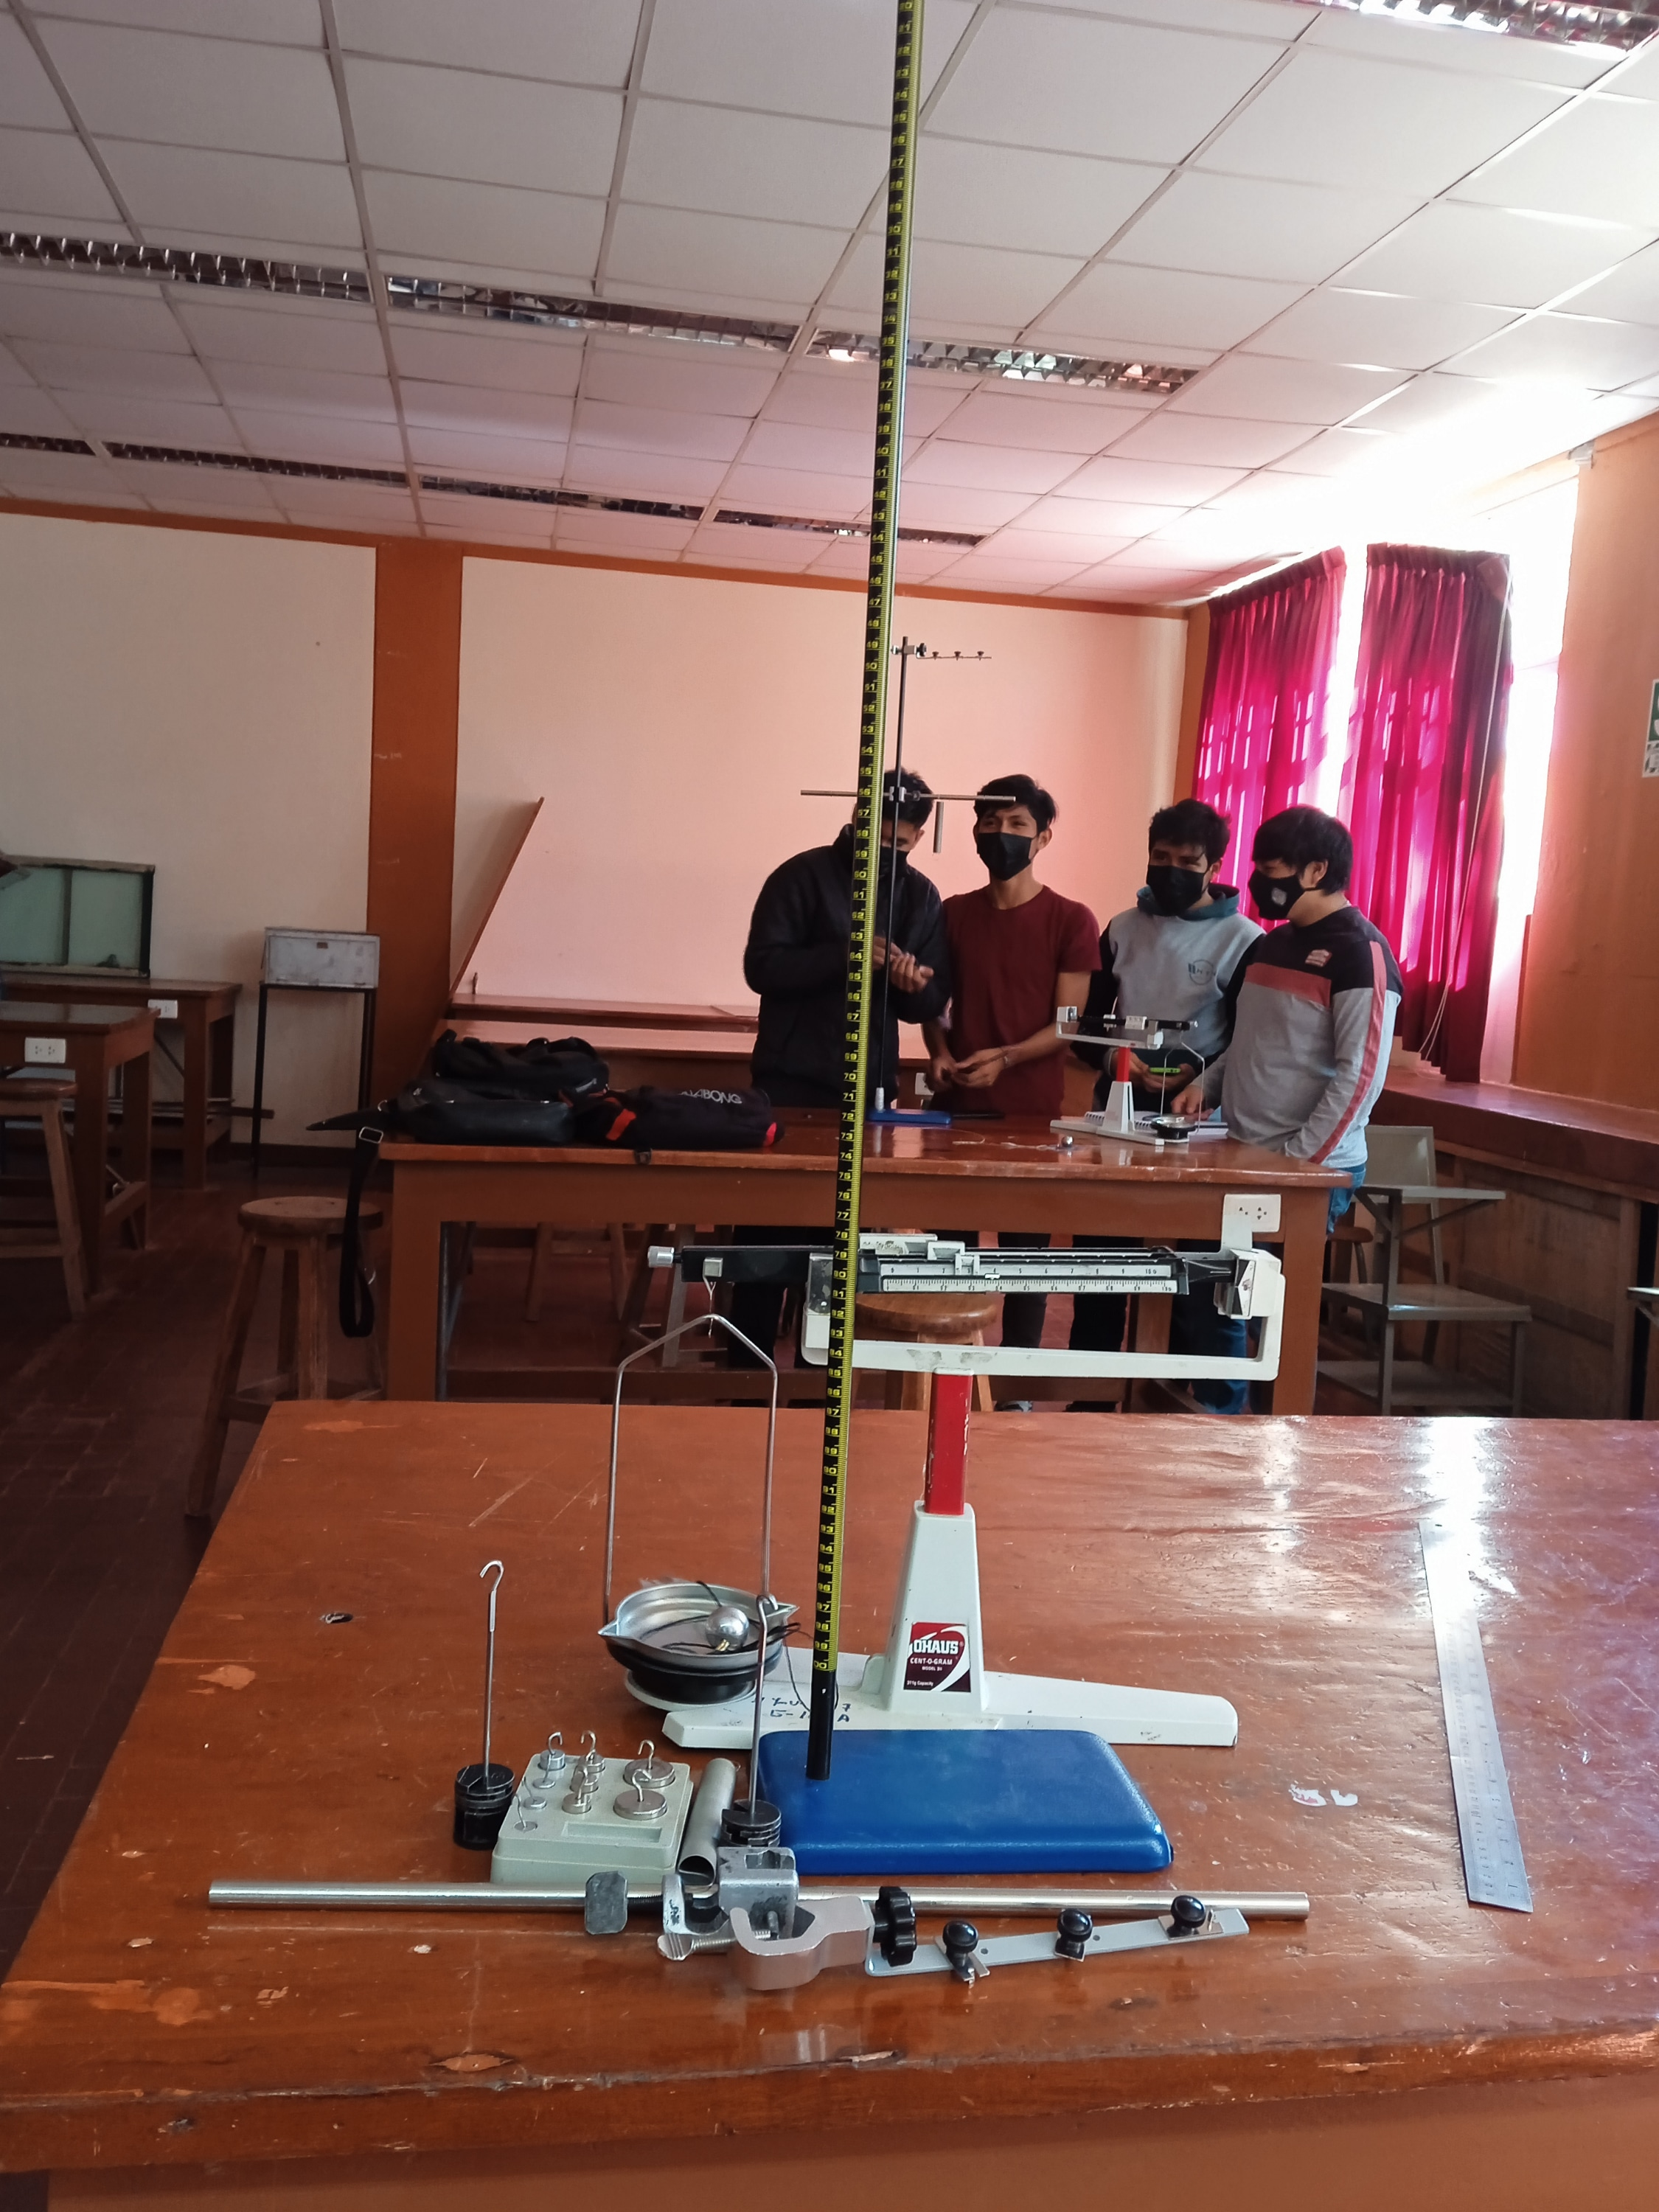
\includegraphics[width=6cm]{Images/materials.jpeg}
		\caption{Materiales utilizados en la práctica de laboratorio.}\label{fig:01}
	\end{figure}

	\begin{figure}[H]
		\centering
		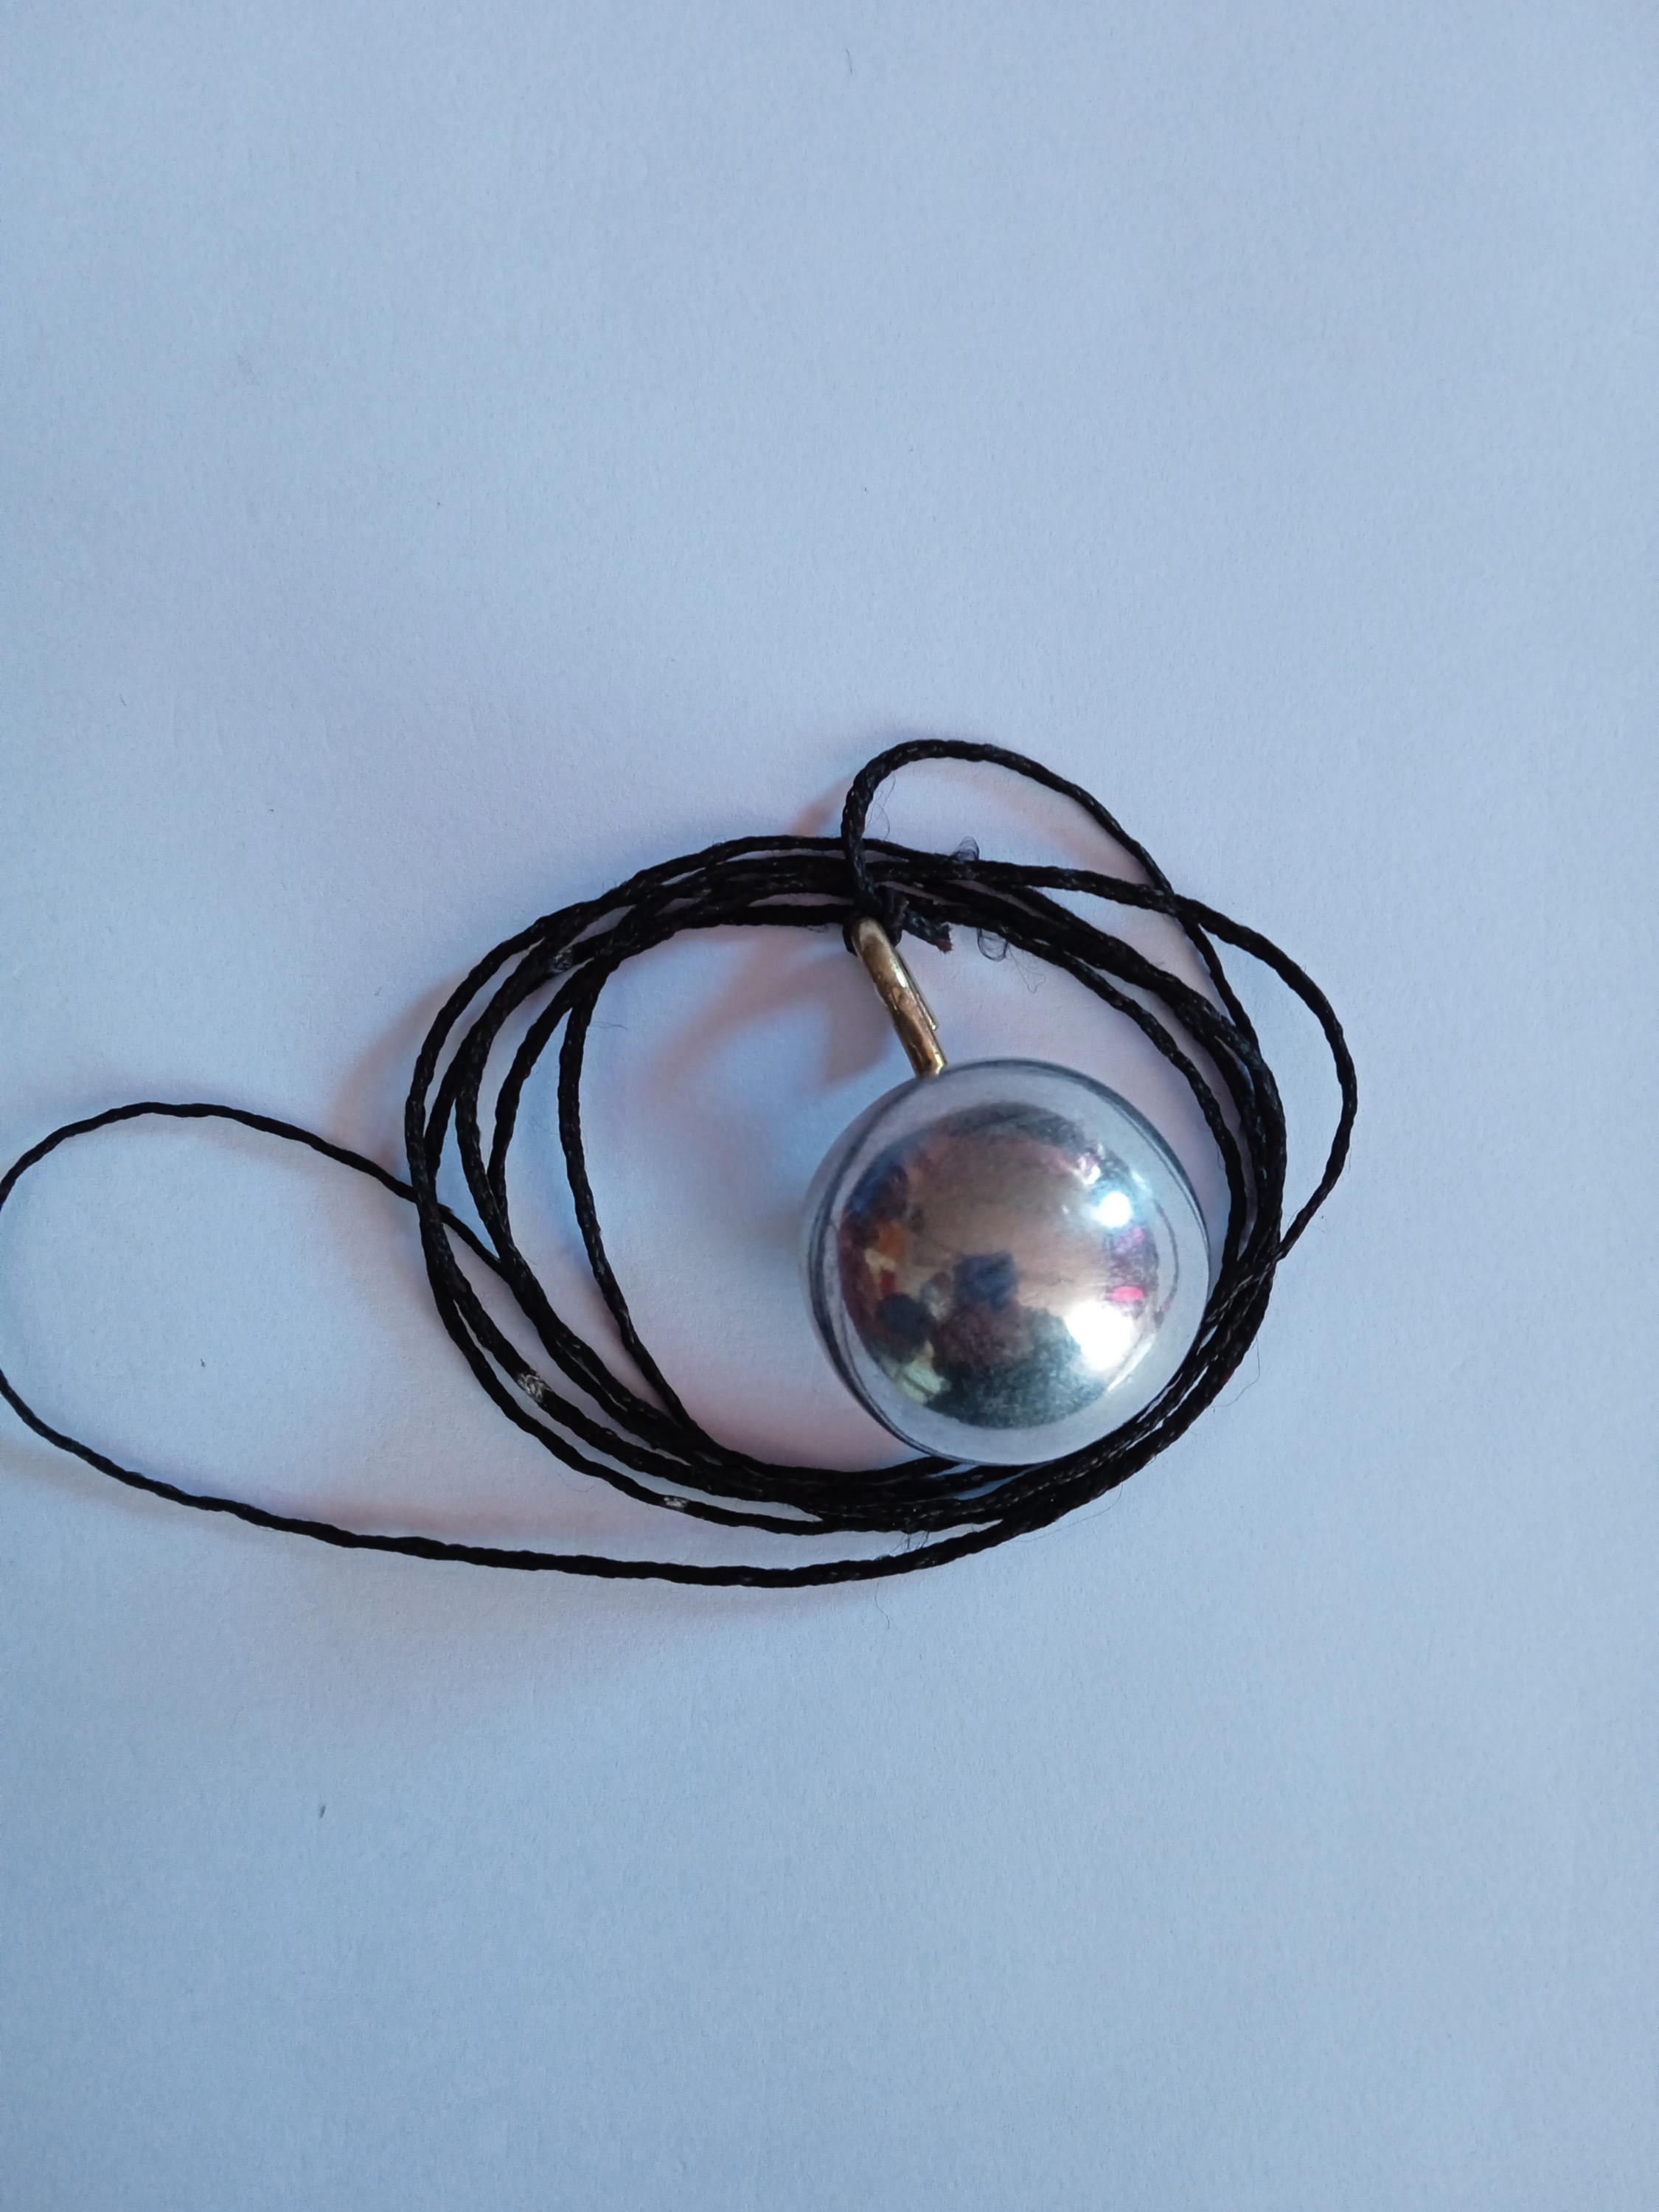
\includegraphics[width=6cm]{Images/masa_hilo.jpeg}
		\caption{Masa (esfera) e hilo.}\label{fig:02}
	\end{figure}
\end{multicols}

%-------------------------------------------------------------------------------------------
\section{Fundamento teórico}
\subsection{Movimiento Armónico Simple (M.A.S)}
\begin{figure}[H]
	\centering
	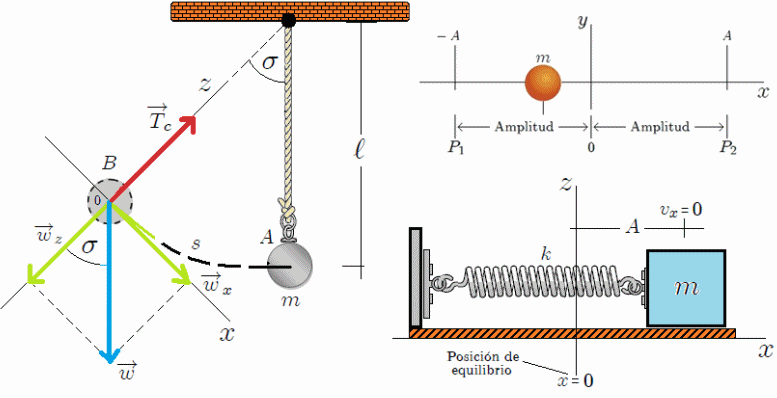
\includegraphics[width=12cm]{Images/fig_02}
	\caption{Movimiento armónico simple.}\label{fig:03}
\end{figure}
El Movimiento Armónico Simple (MAS) es el movimiento periódico más sencillo que se puede analizar, el cual sucede cuando existe una fuerza de restitución $F_R$, la cual es directamente proporcional al desplazamiento x con respecto a un punto equilibrio.
El movimiento armónico simple es la proyección del movimiento circular uniforme sobre un diámetro.
\begin{figure}[H]
	\centering
	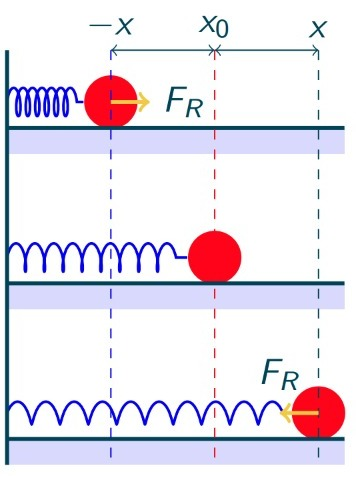
\includegraphics[width=5cm]{Images/fig_i.jpeg}
\end{figure}

\subsubsection{Características del movimiento armónico simple}
\paragraph{Amplitud del movimiento}
\begin{itemize}[label=\textbf{$\bullet$},itemsep=2pt,partopsep=6pt,parsep=6pt]
	\item Se denota con la letra A y se define como la magnitud máxima del desplazamiento con respecto al equilibrio; es decir, el valor máximo de $|x|$ y siempre es positivo.
	\item El rango global del movimiento es 2A.
	\item Las unidades de A depende del fenómeno físico que estemos trabajando.
\end{itemize}
\paragraph{Perido y frecuencia}
\begin{itemize}[label=\textbf{$\bullet$},itemsep=2pt,partopsep=6pt,parsep=6pt]
	\item El periodo se denota con la letra T y se define como el tiempo que tarda en cumplirse un ciclo.
	\item La unidad del periodo en el SI es el segundo, aunque a veces se expresa como segundos por ciclo.
	\item La frecuencia se denota con la letra f, y se define como el número de ciclos por la unidad de tiempo que realiza un movimiento periódico.
	\item La frecuencia se relaciona con el periodo mediante la siguiente relación.
	      \[f=\cfrac{1}{T}\]
	\item La unidad de la frecuencia en el SI es el Hertz ($1hz=$ ciclo/s$=1{s}^{-1}$).
\end{itemize}
\paragraph{Fecuencia angular}
\begin{itemize}[label=\textbf{$\bullet$},itemsep=2pt,partopsep=6pt,parsep=6pt]
	\item La frecuencia angular se denota con la letra $w$, y se define:
	\item La frecuencia representa la rapidezde cambio de una cantidad angular la cual se mide en radianes, de modo que sus unidades son $rad/s$.
\end{itemize}
\subsubsection{Ecuación diferencial del MAS}
\begin{itemize}[label=\textbf{$\bullet$},itemsep=2pt,partopsep=6pt,parsep=6pt]
	\item Si se considera elsistema masa-resorte y se aplica la segunda ley de Newton a la masa m:
	      \[\sum F_x=-kx=ma\]
	\item Usando la definición de la aceleración se tiene:
	      \[-kx=m\cfrac{d^2 x}{dt^2}\]
	\item Finalmente se obtiene la ecuacion diferenacial general del MAS\@.
	      \[\frac{d^2 x}{dt^2}+\omega^2 x=0\]
	      donde la frecuencia angular del sistema se define como
	      \[\omega=\sqrt[]{\cfrac{k}{m}}\]
\end{itemize}
La solución de dicha ecuación diferencial es:
\[x(t)=A\cos (\omega t+ \phi)\]
donde x describe la poisición de la masa y la cosntante $\phi$ es el ángulo de fase, el cual sirve para encontrarlas condiciones iniciales $(x(0)$, $v_x (0)$ y  $a_x(0))$ del movimiento oscilador.
\begin{figure}[H]
	\centering
	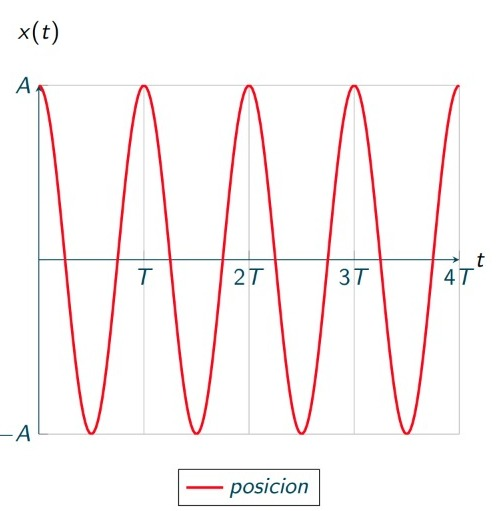
\includegraphics[width=9cm]{Images/min_i.jpeg}
\end{figure}
\subsubsection{Características MAS Sistema masa-resorte}
Para un sistema mas-resorte que describe un MAS las características del movimiento quedan definidas en términos de $\omega$, como por ejemplo.
\begin{itemize}[label=\textbf{$\bullet$},itemsep=2pt,partopsep=6pt,parsep=6pt]
	\item Periodo
	      \[T=\cfrac{2\pi}{\omega}=2\pi \text{ }\sqrt[]{\dfrac{m}{k}}\]
	\item Frecuencia
	      \[f=\cfrac{\omega}{2\pi}=\cfrac{1}{2\pi}\text{ }\sqrt{\cfrac{k}{m}}\]
\end{itemize}
De lo anterior se puede ver que en el MAS descrito por un sistema masa-resorte, el periodo y la frecuencia no dependen de la amplitud.%\ref{fig:04}
\paragraph{Velocidad para un sistema que describe un MAS}
Usando la definición de velocidad se obtiene:
\[v(t)=\cfrac{dx}{dt}=-A\omega \sin (\omega t+\phi)\]
\begin{figure}[H]
	\centering
	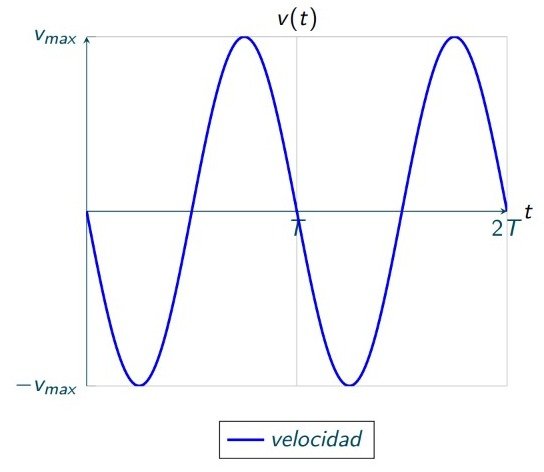
\includegraphics[width=9cm]{Images/min_ii.jpeg}
\end{figure}
\paragraph{Aceleración para una masa que describe un MAS}
Usando la definición de aceleración se obtiene:
\[a(t)=\cfrac{dv}{dt}=-A\omega^2 \cos (\omega t+\phi)\]
\begin{figure}[H]
	\centering
	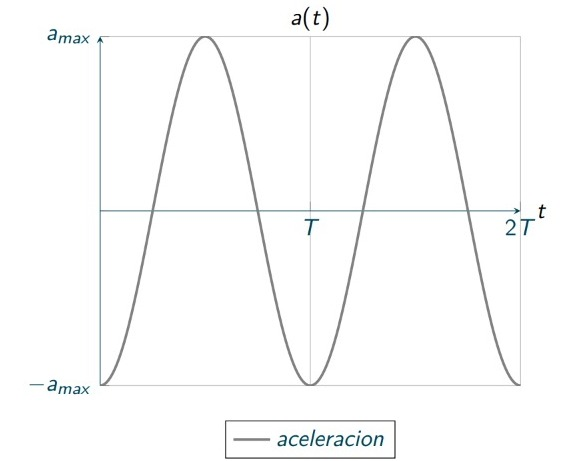
\includegraphics[width=9cm]{Images/min_iii.jpeg}
\end{figure}
%==========================================================================================
\section{Procedimiento y toma de datos}
%-------------------------------------------------------------------------------------------
\subsection{Actividad 1}
\begin{dyNoteImportant}[morado01!20]{azulfor!10}{black!80}{Secuencia de la actividad}
	\begin{enumerate}[label=\itemcirccz{miverde}{\arabic*},itemsep=2pt, leftmargin=0.6cm]
		\item Suspende el resorte y debajo coloque una masa, estire el resorte ligeramente hacia abajo, observe el fenómeno y determine el periodo tomando el tiempo de 10 oscilaciones dos veces.
		\item Discuta con sus compañeros de grupo y calcule la constante k del resorte.
		\item Repita la experiencia para 5 valores de masas diferentes y prepare un cuadro de datos adecuado.
	\end{enumerate}
\end{dyNoteImportant}

\begin{figure}[H]
	\centering
	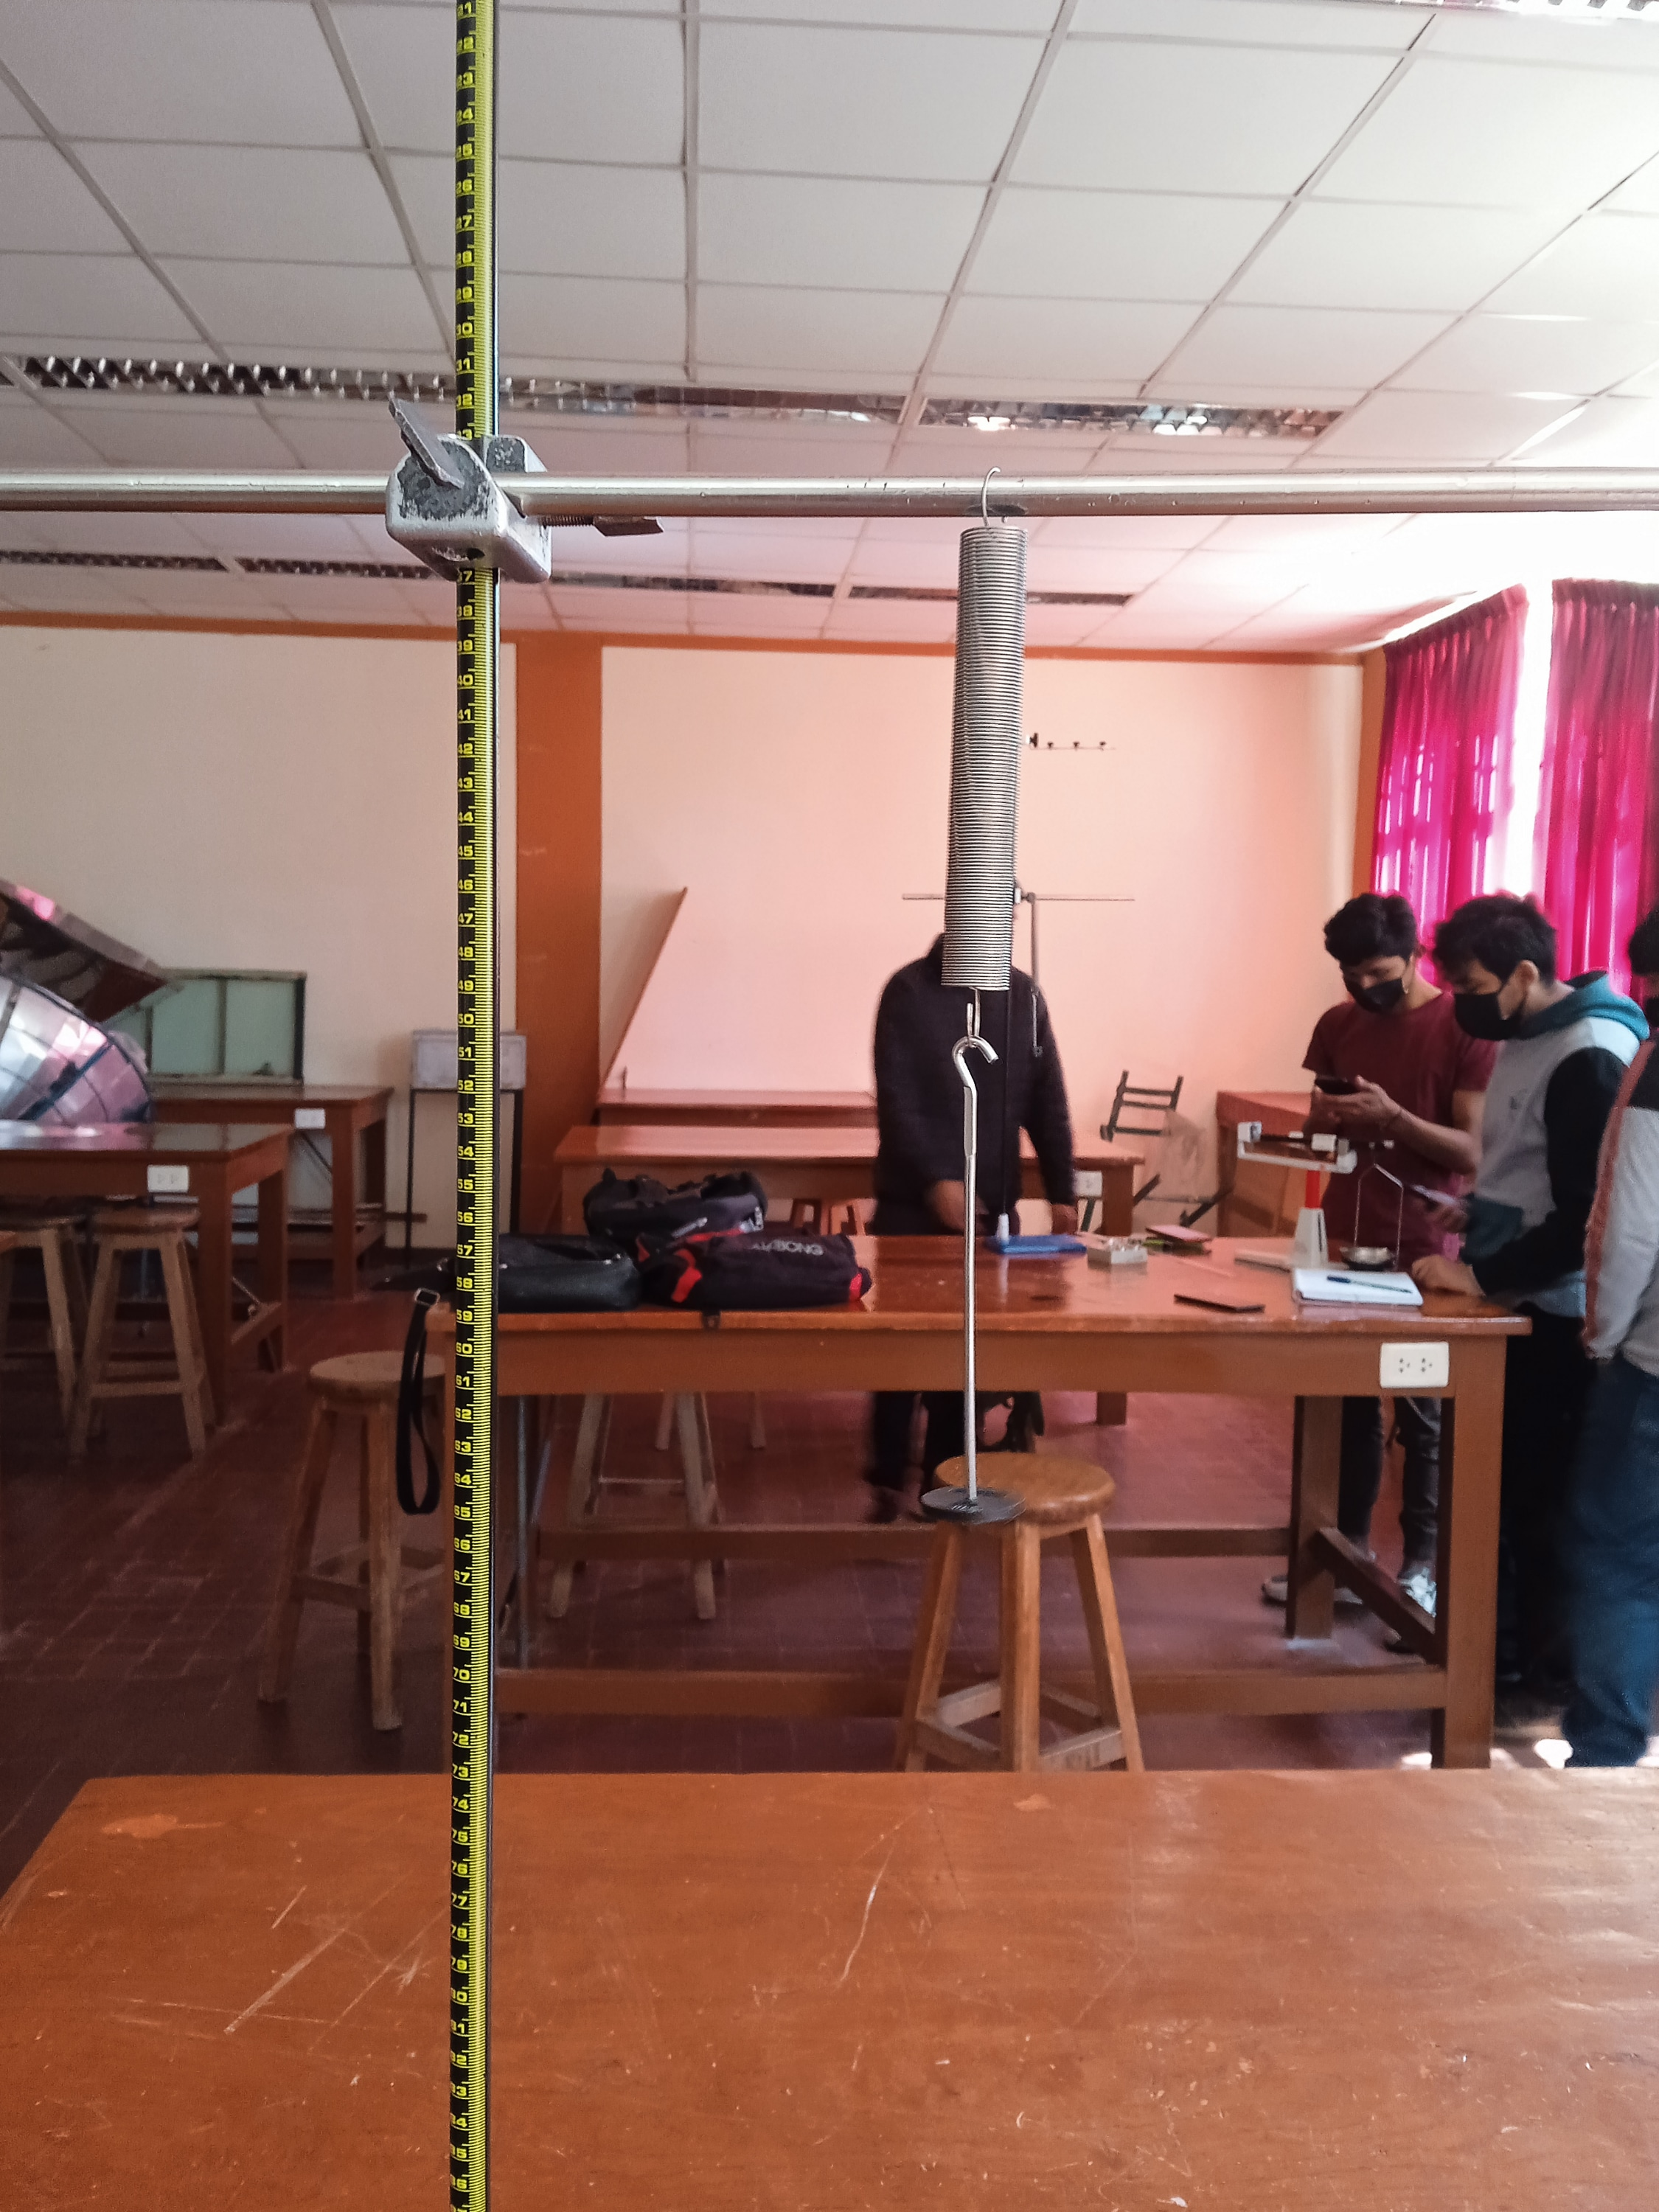
\includegraphics[width=6cm]{Images/spring.jpeg}
	\caption{Experimento MAS masa-resorte.}\label{fig:04}
\end{figure}

\subsubsection{Primer caso}
\begin{enumerate}[label=\bfseries\alph*.-,itemsep=2pt]
	\item \textbf{Calculando el tiempo promedio}
	      \[t_\Delta = \cfrac{t_1+t_2}{2}\]

	      \sdconditions[12cm]{azzul}{Donde:}{%
		      \begin{tabular}{lcl}
			      $t_\Delta$ & \@: & tiempo promedio (en segundos). \\
			      $t_1$      & \@: & tiempo 1 (en segundos).        \\
			      $t_2$      & \@: & tiempo 2 (en segundos).
		      \end{tabular}
	      }

	      \begin{itemize}[label=\textbf{$\bullet$},itemsep=2pt,partopsep=6pt]
		      \item Para el primer evento.
		            \[t_{\Delta{1}}=\cfrac{4.58+4.53}{2}=4.56\]
		      \item Para el segundo evento.
		            \[t_{\Delta{2}}=\cfrac{6.02+6.03}{2}=6.03\]
		      \item Para el tercer evento.
		            \[t_{\Delta{3}}=\cfrac{7.17+7.23}{2}=7.20\]
		      \item Para el cuarto evento.
		            \[t_{\Delta{4}}=\cfrac{8.24+8.18}{2}=8.21\]
		      \item Para el quinto evento.
		            \[t_{\Delta{5}}=\cfrac{9.09+9.13}{2}=9.11\]
	      \end{itemize}
	\item \textbf{Calculando el periodo}
	      \[T = \dfrac{t_\Delta}{10}\]
	      \begin{itemize}[label=\textbf{$\bullet$},itemsep=2pt,partopsep=6pt]
		      \item Para el primer evento.
		            \[T_1 = \dfrac{4.56}{10}=0.46\]
		      \item Para el segundo evento.
		            \[T_2 = \dfrac{6.03}{10}=0.60\]
		      \item Para el tercer evento.
		            \[T_3 = \dfrac{7.20}{10}=0.72\]
		      \item Para el cuarto evento.
		            \[T_4 = \dfrac{8.21}{10}=0.82\]
		      \item Para el quinto evento.
		            \[T_5 = \dfrac{9.11}{10}=0.91\]
	      \end{itemize}

	\item \textbf{Calculando la constante de rigidez}
	      \[k= \cfrac{4\pi^2 m}{T^2}\]

	      \sdconditions[12cm]{azzul}{Donde:}{%
		      \begin{tabular}{lcl}
			      $k$ & \@: & constante de rigidez.  \\
			      $m$ & \@: & masa (en Kilogramos).  \\
			      $T$ & \@: & periodo (en segundos).
		      \end{tabular}
	      }

	      \begin{itemize}[label=\textbf{$\bullet$},itemsep=2pt,partopsep=6pt]
		      \item Para el primer evento.
		            \[k_1= \cfrac{4\times\pi^2\times{0.04}}{{0.46}^2}=7.61\]
		      \item Para el segundo evento.
		            \[k_2= \cfrac{4\times\pi^2\times{0.07}}{{0.6}^2}=7.61\]
		      \item Para el tercer evento.
		            \[k_3= \cfrac{4\times\pi^2\times{0.1}}{{0.72}^2}=7.62\]
		      \item Para el cuarto evento.
		            \[k_4= \cfrac{4\times\pi^2\times{0.13}}{{0.82}^2}=7.61\]
		      \item Para el quinto evento.
		            \[k_5= \cfrac{4\times\pi^2\times{0.16}}{{0.91}^2}=7.61\]
	      \end{itemize}
\end{enumerate}

\subsubsection{Segundo caso}
\begin{enumerate}[label=\bfseries\alph*.-,itemsep=2pt]
	\item \textbf{Calculando la variación de x}
	      \[\Delta x= \cfrac{x_f-x_i}{2}\]
	      \begin{itemize}[label=\textbf{$\bullet$},itemsep=2pt,partopsep=6pt,parsep=6pt]
		      \item Para el primer evento.
		            \[\Delta x_1= \cfrac{15.75-10.6}{2}=2.58cm<>0.3m\]
		      \item Para el segundo evento.
		            \[\Delta x_2= \cfrac{19.6-10.6}{2}=4.5cm<>0.05m\]
		      \item Para el tercer evento.
		            \[\Delta x_3= \cfrac{23.46-10.6}{2}=6.43cm<>0.06m\]
		      \item Para el cuarto evento.
		            \[\Delta x_4= \cfrac{27.33-10.6}{2}=8.37cm<>0.08m\]
		      \item Para el quinto evento.
		            \[\Delta x_5= \cfrac{31.2-10.6}{2}=10.3cm<>0.10m\]
	      \end{itemize}

	\item \textbf{Calculando la constante de rigidez}
	      \[k= \cfrac{F}{x}\]

	      \sdconditions[12cm]{azzul}{Donde:}{%
		      \begin{tabular}{lcl}
			      $k$ & \@: & constante de rigidez.    \\
			      $F$ & \@: & fuerza (en newtons).     \\
			      $x$ & \@: & deformación (en metros).
		      \end{tabular}
	      }
	      \begin{itemize}[label=\textbf{$\bullet$},itemsep=2pt,partopsep=6pt,parsep=6pt]
		      \item Para el primer evento.
		            \[k_1= \cfrac{0.04\times{9.8}}{x}=7.61\]
		      \item Para el segundo evento.
		            \[k_2= \cfrac{0.07\times{9.8}}{x}=7.62\]
		      \item Para el tercer evento.
		            \[k_3= \cfrac{0.1\times{9.8}}{x}=7.62\]
		      \item Para el cuarto evento.
		            \[k_4= \cfrac{0.13\times{9.8}}{x}=7.62\]
		      \item Para el quinto evento.
		            \[k_5= \cfrac{0.16\times{9.8}}{x}=7.61\]
	      \end{itemize}
\end{enumerate}

%-------------------------------------------------------------------------------------------
\subsection{Actividad 2}
\begin{dyNoteImportant}[morado01!20]{azulfor!10}{black!80}{Secuencia de la actividad}
	\begin{enumerate}[label=\itemcirccz{miverde}{\arabic*},itemsep=2pt, leftmargin=0.6cm]
		\item Mida la longitud del péndulo y el periodo del péndulo tomando el tiempo de 10 oscilaciones dos veces, repita esta experiencia para 5 masas diferentes y anote en la tabla.
		\item Varíe la longitud del péndulo 5 veces y determine el periodo tomando el tiempo de 10 oscilaciones.
		\item Grafique $T^2$ en función a $L$ y calcule a partir de ella $g$.
		\item Tome el péndulo de una longitud determinada, variando cinco veces la masa, mide dos veces en cada caso, el tiempo que tarda 10 oscilaciones.
	\end{enumerate}
\end{dyNoteImportant}

\begin{figure}[H]
	\centering
	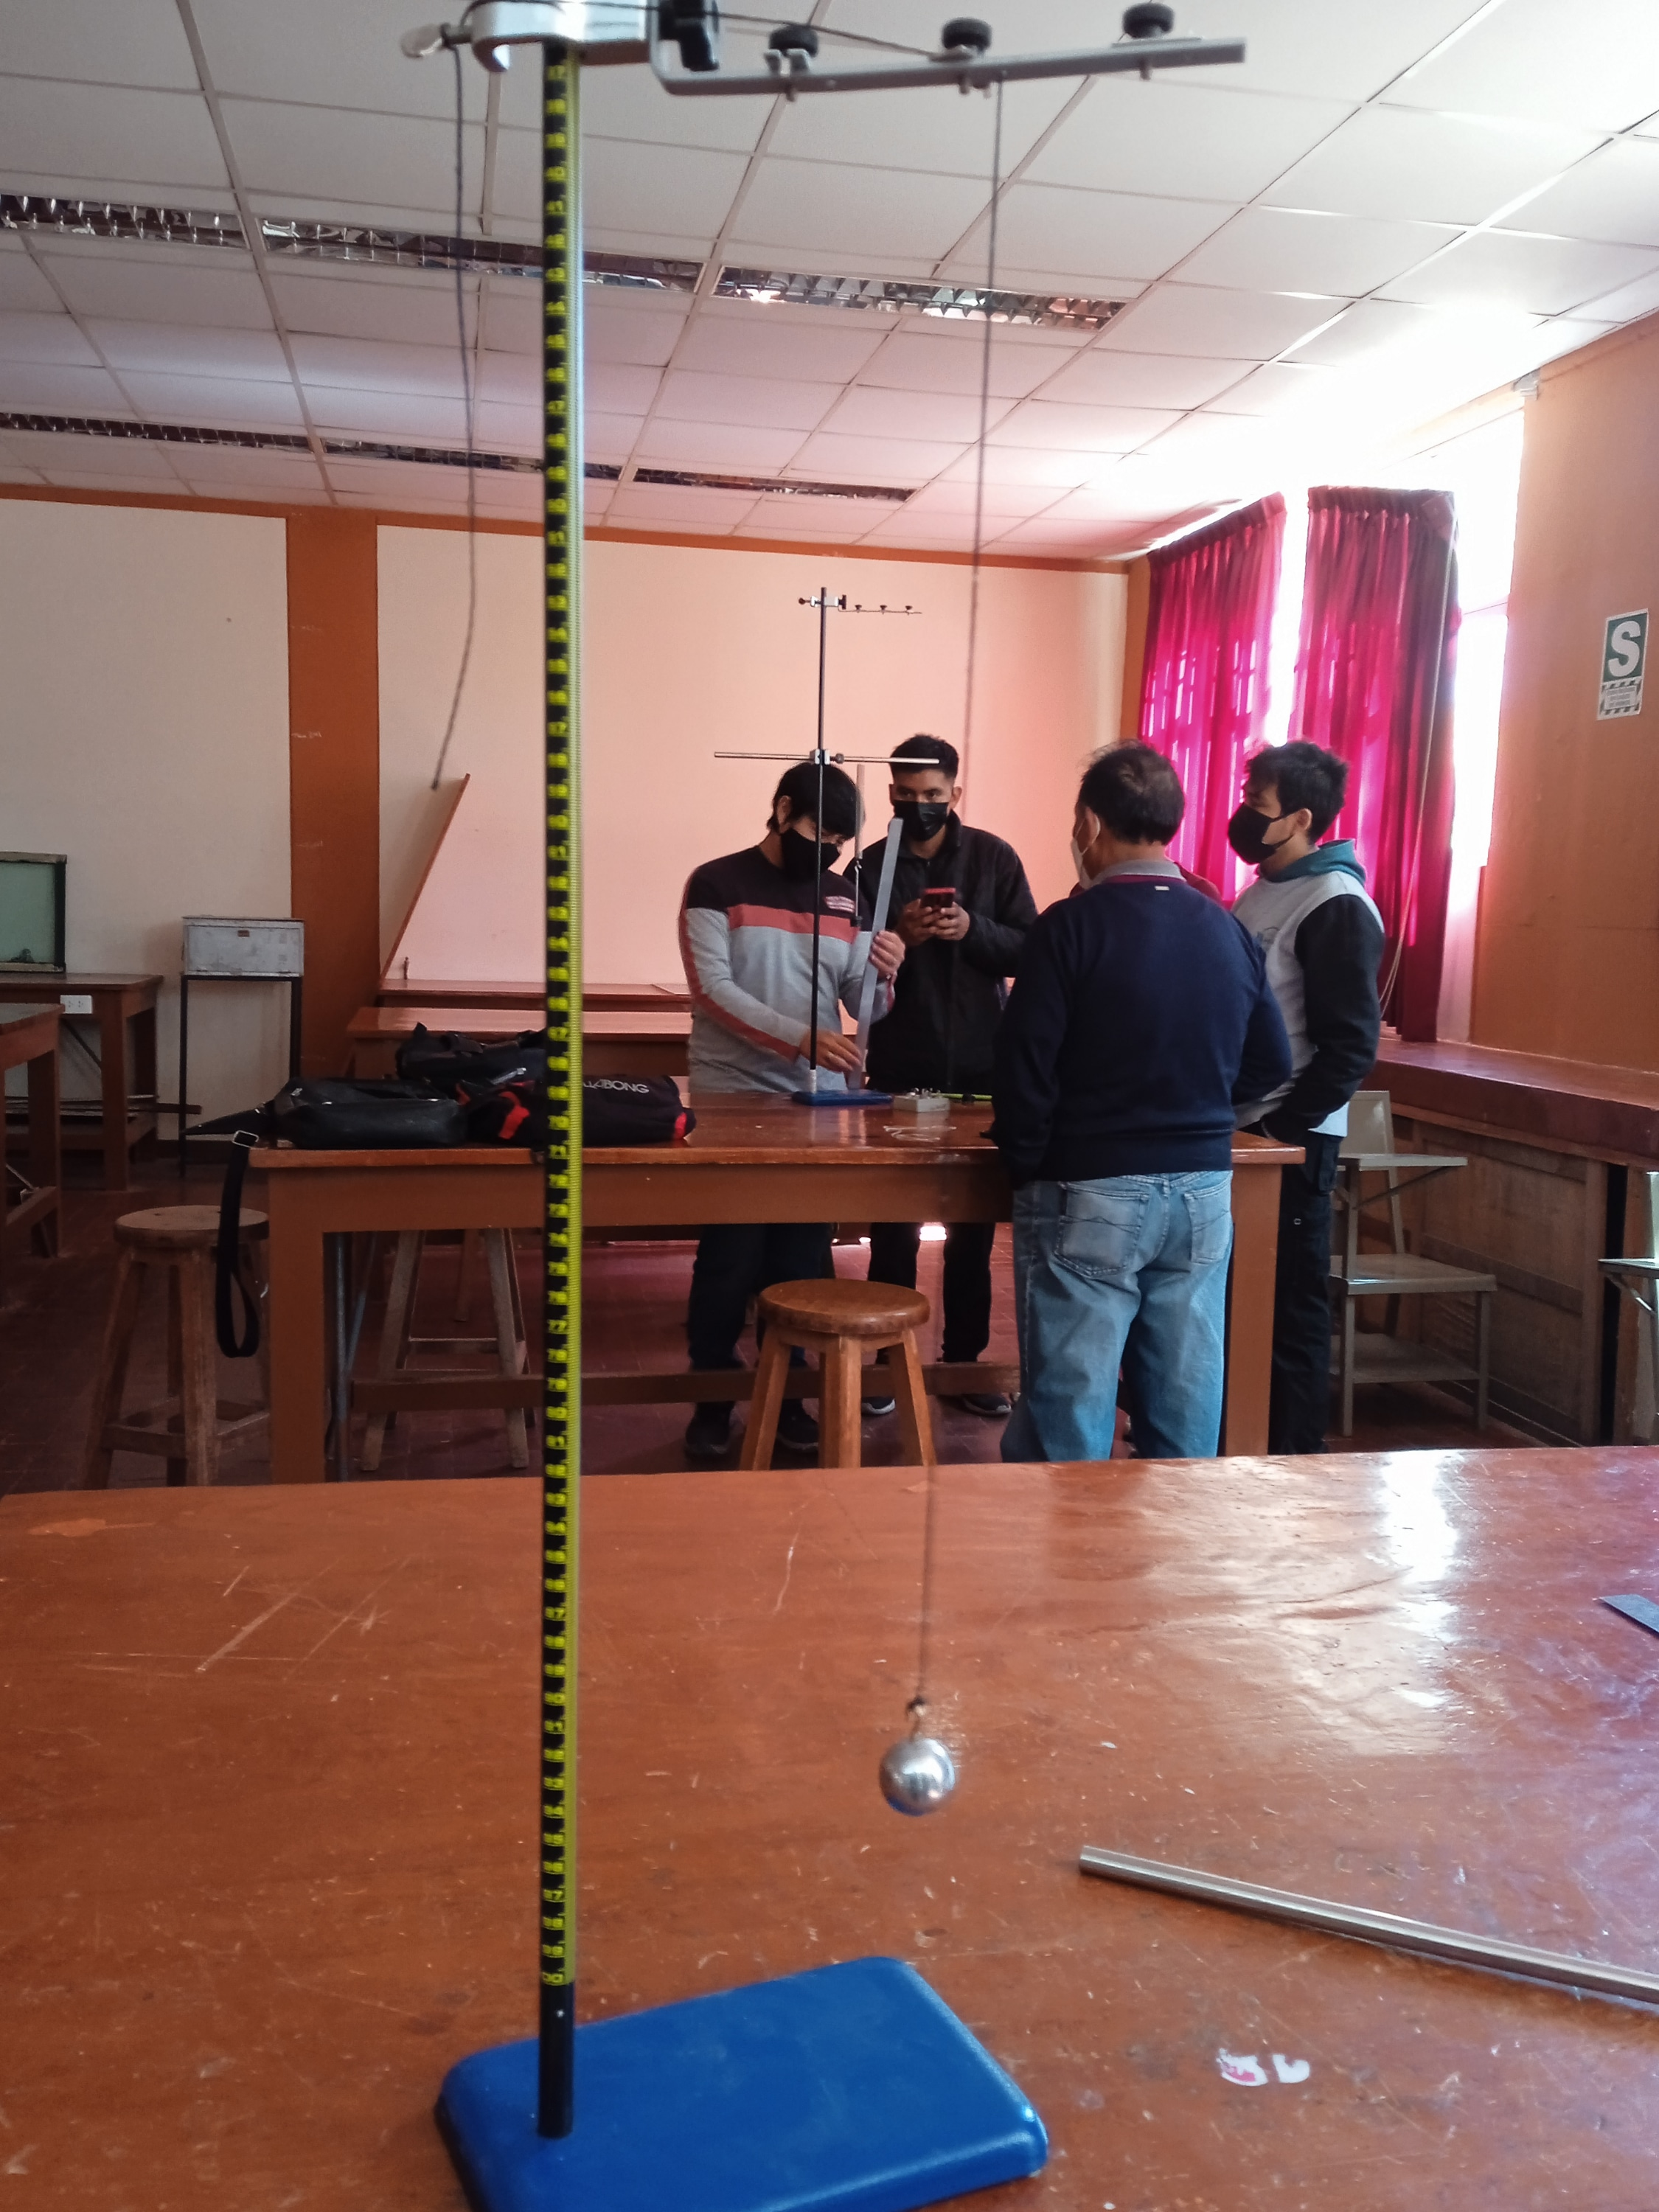
\includegraphics[width=6cm]{Images/pendulum.jpeg}
	\caption{Experimento MAS pendulo simple.}\label{fig:05}
\end{figure}

\subsubsection{Para la longitud constante}
\begin{enumerate}[label=\bfseries\alph*.-,itemsep=2pt]
	\item \textbf{Calculando el tiempo promedio}
	      \[t_\Delta = \cfrac{t_1+t_2}{2}\]
	      \begin{itemize}[label=\textbf{$\bullet$},itemsep=2pt,partopsep=6pt,parsep=6pt]
		      \item Para el primer  evento.
		            \[t_{\Delta{1}}=\cfrac{17.45+17.40}{2}=17.43\]
		      \item Para el segundo evento.
		            \[t_{\Delta{2}}=\cfrac{17.41+17.38}{2}=17.4\]
		      \item Para el tercer  evento.
		            \[t_{\Delta{3}}=\cfrac{17.45+17.55}{2}=17.5\]
		      \item Para el cuarto  evento.
		            \[t_{\Delta{4}}=\cfrac{17.42+17.53}{2}=17.48\]
		      \item Para el quinto  evento.
		            \[t_{\Delta{5}}=\cfrac{17.42+17.50}{2}=17.46\]
	      \end{itemize}

	\item \textbf{Calculando el periodo}
	      \[T = \dfrac{t_\Delta}{10}\]
	      \begin{itemize}[label=\textbf{$\bullet$},itemsep=2pt,partopsep=6pt,parsep=6pt]
		      \item Para el primer evento.
		            \[T_1 = \dfrac{17.43}{10}=1.74\]
		      \item Para el segundo evento.
		            \[T_2 = \dfrac{17.4}{10}=1.74\]
		      \item Para el tercer evento.
		            \[T_3 = \dfrac{17.5}{10}=1.75\]
		      \item Para el cuarto evento.
		            \[T_4 = \dfrac{17.48}{10}=1.75\]
		      \item Para el quinto evento.
		            \[T_5 = \dfrac{17.46}{10}=1.75\]
	      \end{itemize}

	\item \textbf{Calculando la aceleración de la gravedad}
	      \[g= \cfrac{4\pi^2L}{T^2}\]
	      \begin{itemize}[label=\textbf{$\bullet$},itemsep=2pt,partopsep=6pt,parsep=6pt]
		      \item Para el primer evento.
		            \[g_1= \cfrac{4\times\pi^2\times{0.75}}{{1.74}^2}=9.77\]
		      \item Para el segundo evento.
		            \[g_2= \cfrac{4\times\pi^2\times{0.75}}{{1.74}^2}=9.77\]
		      \item Para el tercer evento.
		            \[g_3= \cfrac{4\times\pi^2\times{0.75}}{{1.75}^2}=9.66\]
		      \item Para el cuarto evento.
		            \[g_4= \cfrac{4\times\pi^2\times{0.75}}{{1.75}^2}=9.66\]
		      \item Para el quinto evento.
		            \[g_5= \cfrac{4\times\pi^2\times{0.75}}{{1.75}^2}=9.66\]
	      \end{itemize}
\end{enumerate}

\subsubsection{Para la masa constante}
\begin{enumerate}[label=\bfseries\alph*.-,itemsep=2pt]
	\item \textbf{Calculando el tiempo promedio}
	      \[t_\Delta = \cfrac{t_1+t_2}{2}\]
	      \begin{itemize}[label=\textbf{$\bullet$},itemsep=2pt,partopsep=6pt,parsep=6pt]
		      \item Para el primer  evento.
		            \[t_{\Delta{1}}=\cfrac{17.43+17.58}{2}=17.51\]
		      \item Para el segundo evento.
		            \[t_{\Delta{2}}=\cfrac{15.51+15.60}{2}=15.56\]
		      \item Para el tercer  evento.
		            \[t_{\Delta{3}}=\cfrac{13.55+13.47}{2}=13.51\]
		      \item Para el cuarto  evento.
		            \[t_{\Delta{4}}=\cfrac{11.15+11.06}{2}=11.11\]
		      \item Para el quinto  evento.
		            \[t_{\Delta{5}}=\cfrac{7.95+7.64}{2}=7.8\]
	      \end{itemize}

	\item \textbf{Calculando el periodo}
	      \[T = \dfrac{t_\Delta}{10}\]
	      \begin{itemize}[label=\textbf{$\bullet$},itemsep=2pt,partopsep=6pt,parsep=6pt]
		      \item Para el primer evento.
		            \[T_1 = \dfrac{17.51}{10}=1.75\]
		      \item Para el segundo evento.
		            \[T_2 = \dfrac{15.56}{10}=1.56\]
		      \item Para el tercer evento.
		            \[T_3 = \dfrac{13.51}{10}=1.35\]
		      \item Para el cuarto evento.
		            \[T_4 = \dfrac{11.11}{10}=1.11\]
		      \item Para el quinto evento.
		            \[T_5 = \dfrac{7.8}{10}=0.78\]
	      \end{itemize}

	\item \textbf{Calculando la aceleración de la gravedad}
	      \[g= \cfrac{4\pi^2L}{T^2}\]
	      \begin{itemize}[label=\textbf{$\bullet$},itemsep=2pt,partopsep=6pt,parsep=6pt]
		      \item Para el primer evento.
		            \[g_1= \cfrac{4\times\pi^2\times{0.75}}{{1.75}^2}=9.7\]
		      \item Para el segundo evento.
		            \[g_2= \cfrac{4\times\pi^2\times{0.60}}{{1.56}^2}=9.7\]
		      \item Para el tercer evento.
		            \[g_3= \cfrac{4\times\pi^2\times{0.45}}{{1.35}^2}=9.7\]
		      \item Para el cuarto evento.
		            \[g_4= \cfrac{4\times\pi^2\times{0.30}}{{1.11}^2}=9.6\]
		      \item Para el quinto evento.
		            \[g_5= \cfrac{4\times\pi^2\times{0.15}}{{0.78}^2}=9.7\]
	      \end{itemize}
\end{enumerate}

%==========================================================================================
\section{Tabla y resultados}
\begin{table}[H]
	\centering
	\parbox{10cm}{%
		\caption{Cálculo de la constante de rigidez ($k$).}\label{tab:03}}\\
	\sdconditions[12cm]{azzul}{Para:}{%
		\begin{tabular}{lcl}
			$m$   & \@: & Masa (en kg).                       \\
			$t_1$, $t_2$ y $t_\Delta$ & \@: & Tiempo (en segundos). \\
			$T$ & \@: & Periodo (en segundos). \\
			$K$   & \@: & Constante ed rigidez (en $N/m$).
		\end{tabular}
	}
	\begin{tabular}{C{0.5cm}C{1cm}C{1cm}C{1cm}C{1cm}C{1cm}C{1cm}}
		\hline
		\rowcolor{gray!10}$N$ & $m$    & $t_1$  & $t_2$  & $t_\Delta$ & $T$    & $K$    \\
		\hline
		1                     & $0.4$  & $4.58$ & $4.53$ & $4.56$     & $0.46$ & $7.61$ \\
		2                     & $0.7$  & $6.02$ & $6.03$ & $6.03$     & $0.60$ & $7.61$ \\
		3                     & $0.1$  & $7.17$ & $7.23$ & $7.20$     & $0.72$ & $7.62$ \\
		4                     & $0.13$ & $8.24$ & $8.18$ & $8.21$     & $0.82$ & $7.61$ \\
		5                     & $0.16$ & $9.09$ & $9.13$ & $9.11$     & $0.91$ & $7.61$ \\
		\midrule
	\end{tabular}
\end{table}
\begin{table}[H]
	\centering
	\parbox{7cm}{%
		\caption{Cálculo de la constante de rigidez ($k$).}\label{tab:04}}\\
	\sdconditions[12cm]{azzul}{Para:}{%
		\begin{tabular}{lcl}
			$F$   & \@: & Fuerza (en Newtons)                       \\
			$x_i$ & \@: & Resorte sin deformación (en centímetros). \\
			$x_f$ & \@: & Resorte con deformación (en centímetros). \\
			$x_m$ & \@: & Deformación (en metros).                  \\
			$K$   & \@: & Constante ed rigidez (en $N/m$).
		\end{tabular}
	}
	\begin{tabular}{C{0.5cm}C{1cm}C{1cm}C{1cm}C{1cm}C{1cm}}
		\hline
		\rowcolor{gray!10}$N$ & $F$    & $x_i$  & $x_f$   & $x_m$  & $K$    \\ \hline
		1                     & $0.04$ & $10.6$ & $15.75$ & $0.04$ & $7.61$ \\
		2                     & $0.07$ & $10.6$ & $19.6$  & $0.05$ & $7.62$ \\
		3                     & $0.1$  & $10.6$ & $23.46$ & $0.06$ & $7.62$ \\
		4                     & $0.13$ & $10.6$ & $27.33$ & $0.08$ & $7.62$ \\
		5                     & $0.16$ & $10.6$ & $31.2$  & $0.10$ & $7.61$ \\
		\midrule
	\end{tabular}
\end{table}
%====================================================$
\begin{table}[H]
	\centering
	\parbox{9cm}{%
		\caption{Cálculo de la gravedad.}\label{tab:01}}\\
	\sdconditions[12cm]{azzul}{Para:}{%
		\begin{tabular}{lcl}
			$m_1$                   & \@: & $23.35$gr. $<>0.03$kg. \\
			$t_1, t_2$ y $t_\Delta$ & \@: & tiempo (en seundos).   \\
			$T$                     & \@: & Periodo (en Hertz).    \\
			$g$                     & \@: & gravedad (en $m/s^2$).
		\end{tabular}
	}
	\begin{tabular}{C{0.35cm}C{1.3cm}C{1cm}C{1cm}C{1cm}C{1cm}C{1cm}}
		\hline
		\rowcolor{gray!10} $N$ & $m$      & $t_1$   & $t_2$   & $t_\Delta $ & $T$    & $g$    \\
		\hline
		1                      & $m_1$    & $17.45$ & $17.40$ & $17.43$     & $1.74$ & $9.77$ \\
		2                      & $m_1+2$  & $17.41$ & $17.38$ & $17.4$      & $1.74$ & $9.77$ \\
		3                      & $m_1+5$  & $17.45$ & $17.55$ & $17.5$      & $1.75$ & $9.66$ \\
		4                      & $m_1+10$ & $17.42$ & $17.53$ & $17.48$     & $1.75$ & $9.66$ \\
		5                      & $m_1+20$ & $17.42$ & $17.50$ & $17.46$     & $1.75$ & $9.66$ \\
		\midrule
	\end{tabular}
\end{table}

\begin{table}[H]
	\centering
	\parbox{10cm}{%
		\caption{Cálculo de la gravedad.}\label{tab:02}}\\
	\sdconditions[12cm]{azzul}{Para:}{%
		\begin{tabular}{lcl}
			$L$                     & \@: & Longitud (en metros)   \\
			$t_1, t_2$ y $t_\Delta$ & \@: & tiempo (en seundos).   \\
			$T$                     & \@: & Periodo (en segundos).    \\
			$g$                     & \@: & gravedad (en $m/s^2$).
		\end{tabular}
	}
	\begin{tabular}{C{0.5cm}C{1cm}C{1cm}C{1cm}C{1cm}C{1cm}C{1cm}}
		\hline
		\rowcolor{gray!10} $N$ & $L$  & $t_1$   & $t_2$   & $t_\Delta$ & $T$    & $g$   \\
		\hline
		1                      & $75$ & $17.43$ & $17.58$ & $17.51$    & $1.75$ & $9.7$ \\
		2                      & $60$ & $15.51$ & $15.60$ & $15.56$    & $1.56$ & $9.7$ \\
		3                      & $45$ & $13.55$ & $13.47$ & $13.51$    & $1.35$ & $9.7$ \\
		4                      & $30$ & $11.15$ & $11.06$ & $11.11$    & $1.11$ & $9.6$ \\
		5                      & $15$ & $ 7.95$ & $ 7.64$ & $ 7.8$     & $0.78$ & $9.7$ \\
		\midrule
	\end{tabular}
\end{table}
%==========================================================================================
\section{Cuestionario}
\begin{enumerate}[itemsep=2pt]
	\item ¿Qué significado tiene la gráfica {\bf T} vs {\bf $\sqrt{m}$} en el experimento de masa resorte?
	El periodo es directamente proporcional a la $\sqrt{m}$, como podemos observar en la figura~\ref{Fig:min}.
	\begin{figure}[H]
		\centering
		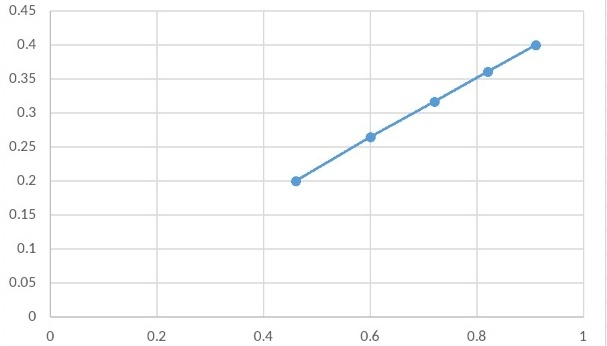
\includegraphics[width=8cm]{Images/min_iv.jpeg}
		\caption{Gráfica $T$ vs $\sqrt{m}$}\label{Fig:min}
	\end{figure}
	\item ¿Qué entiende por MAS?, De los resultados  de la práctica determine la ecuación de movimiento en cada caso.%\cite{ref_05}
	\[x(t)=A\cos(\omega t+ \phi)\]
	\item De acuerdo  a los resultados del experiemnto ¿Cúal es la relación del periodo al variar la masa del péndulo?\\
	No varia, en la fórmula $T=2\pi \sqrt{\tfrac{l}{g}}$, solo depende de la longitud.
\end{enumerate}

%========================================================================================== 
%-------------------------------------
%\begin{center}
	\begin{tabular}{C{0.35cm}C{1.3cm}C{1cm}C{1cm}C{1cm}C{1cm}C{1cm}}
		$N$ & $m$      & $t_1$   & $t_2$   & $t_\Delta $ & $T$    & $g$    \\
		\bottomrule
		1   & $m_i$    & $17.45$ & $17.40$ & $17.43$     & $1.74$ & $9.77$ \\
		2   & $m_1+2$  & $17.41$ & $17.38$ & $17.4$      & $1.74$ & $9.77$ \\
		3   & $m_1+5$  & $17.45$ & $17.55$ & $17.5$      & $1.75$ & $9.66$ \\
		4   & $m_1+10$ & $17.42$ & $17.53$ & $17.48$     & $1.75$ & $9.66$ \\
		5   & $m_1+20$ & $17.42$ & $17.50$ & $17.46$     & $1.75$ & $9.66$
	\end{tabular}
\end{center}

\begin{center}
	\begin{tabular}{C{0.5cm}C{1cm}C{1cm}C{1cm}C{1cm}C{1cm}C{1cm}}
		$N$ & $L$  & $t_1$   & $t_2$   & $t_\Delta$ & $T$    & $g$   \\
		\bottomrule
		1   & $75$ & $17.43$ & $17.58$ & $17.51$    & $1.75$ & $9.7$ \\
		2   & $60$ & $15.51$ & $15.60$ & $15.56$    & $1.56$ & $9.7$ \\
		3   & $45$ & $13.55$ & $13.47$ & $13.51$    & $1.35$ & $9.7$ \\
		4   & $30$ & $11.15$ & $11.06$ & $11.11$    & $1.11$ & $9.6$ \\
		5   & $15$ & $ 7.95$ & $ 7.64$ & $ 7.8$     & $0.78$ & $9.7$
	\end{tabular}
\end{center}
$====================================================$
\begin{center}
	\begin{tabular}{C{0.5cm}C{1cm}C{1cm}C{1cm}C{1cm}C{1cm}C{1cm}}
		$N$ & $m$   & $t_1$  & $t_2$  & $t_\Delta$ & $T$    & $K$    \\
		\bottomrule
		1   & $0.4$ & $4.58$ & $4.53$ & $4.56$     & $0.46$ & $7.61$ \\
		2   & $0.7$ & $6.02$ & $6.03$ & $6.03$     & $0.60$ & $7.61$ \\
		3   & $0.1$ & $7.17$ & $7.23$ & $7.20$     & $0.72$ & $7.62$ \\
		4   & $0.13$ & $8.24$ & $8.18$ & $8.21$     & $0.82$ & $7.61$ \\
		5   & $0.16$ & $9.09$ & $9.13$ & $9.11$     & $0.91$ & $7.61$
	\end{tabular}
\end{center}

\begin{center}
	\begin{tabular}{C{0.5cm}C{1cm}C{1cm}C{1cm}C{1cm}}
		$N$ & $F$    & $x_i$  & $x_f$   & $K$    \\
		\bottomrule
		1   & $0.04$ & $10.6$ & $15.75$ & $7.61$ \\
		2   & $0.07$ & $10.6$ & $19.6$  & $7.62$ \\
		3   & $0.1$  & $10.6$ & $23.46$ & $7.62$ \\
		4   & $0.13$ & $10.6$ & $27.33$ & $7.62$ \\
		5   & $0.16$ & $10.6$ & $31.2$  & $7.61$
	\end{tabular}
\end{center}
%-------------------------------------
\nocite{*}
\printbibliography[title={Bibliografía},heading=bibintoc]
\end{document} 